%!TEX root = main.tex
\chapter{Analysis of Short-Term Outdoor Photometric Stereo}     % numéroté

\label{ch1}

\section{Introduction}

Photometric stereo has been studied extensively in the past decades, especially on how to deal with various lighting conditions~\cite{alldrin-cvpr-08,basri-ijcv-07,johnson-cvpr-11,oxholm-eccv-12,ackermann-cvpr-12,abrams-eccv-12}. Most of the work on this topic has been done in the laboratory, where illumination is controlled. When trying to apply the technique outdoor, where the illumination is uncontrolled,
(\eg,~\cite{sun-ivc-07,jiang-bunke-sp-91,klaudiny-prl-14,shen-pg-14})
we realized that the sun when modeled as a point light source, does not offer enough variability throughout a single day to robustly solve the PS problem. To circumvent this issue, people proposed to capture for extended amount of time in order to have enough lighting diversity to constrain sufficiently the problem~\cite{ackermann-cvpr-12,abrams-eccv-12}. Although previous work have presented sensitivity analyses for standard PS with point light sources, so far as we know, the case of outdoor PS with more complex illumination models has received little attention. 

A promising approach to answer this question is to use more elaborate models of illumination---high dynamic range (HDR) environment maps~\cite{reinhard-book-05}---as input to outdoor PS. Promising results have been reported in~\cite{yu-iccp-13} for outdoor images taken within an interval of just eight hours within a single day. However, the quality of outdoor results is reported to be inferior to that obtained in indoor environments, the decline being attributed to modest variation in sunlight. This observation leads to many interesting, unanswered questions: had the sun path and atmosphere conditions been different on that day, could the quality of their results have been better? What is the minimum time interval required to obtain good results in outdoor PS? Is a full day of observations enough and/or necessary to obtain good results in outdoor PS? Or could similar results be obtained over a shorter time interval (say, 1 hour)? If so, what should be happening in the sky over that time interval? Besides easing the requirements on data capture, these questions are also important in that, in future work, they could extend the applicability of outdoor PS to new scenarios (\eg, to more quickly capture non-static outdoor objects that show gradual changes in shape or appearance over time). 

% TODO: maybe move the sentence above to discussion only? We want to show the importance/impact of asking these questions, but we don't want to disappoint the reviewers by not showing dynamic PS results. Maybe this is ok as it is?

In this chapter\footnote{Originally published in~\cite{holdgeoffroy-iccp-15,holdgeoffroy-3dv-15}.}, we present the first answers to the questions above. Here, we seek to determine the relationship between expected surface reconstruction performance and photometric cues available outdoors over the course of the day. Our main goal is to assess the \emph{reconstructibility} of surface patches as a function of their orientation and the illumination conditions, given a set of HDR environment maps captured throughout a single day or less. To achieve this goal, we use a large database of natural, outdoor illumination (sky probes), which we will discuss first. Then, a detailed look at the conditions under which normals can be reconstructed reliably will be presented, followed by an analysis of surface reconstruction stability. Finally, we explore the occurrence of these conditions over the course of a single day and whether PS can be applied over intervals that span less than one day. 

%\section{Outdoor lighting conditions analysis}

%To explore the richness of natural illumination in the context of Photometric Stereo (PS), we exploit the database of outdoor HDR environment maps detailed in the last section, which provides a rich sampling of the variability of outdoor illumination. To ensure the data is properly aligned temporally, only images that were captured during a continuous 6 hour time interval on each of these days, from 10{:}30 until 16{:}30, are considered. Through a theoretical analysis (inspired by \cite{sun-ivc-07}) and supported by an extensive empirical evaluation as well as a preliminary quantitative validation, we derive confidence intervals that allow us to predict when surface normals can be reconstructed more accurately and solely from the photometric cue. Instead of focusing exclusively on sun position~\cite{shen-pg-14}, our analysis incorporates the influence of all components of natural lighting: sun, sky, clouds, etc., as well as noise and surface albedo. 

%In the rest of this chapter, we explore the conditions in which PS may or may not work, when faced with the challenging case of uncontrollable outdoor illumination. 

% Or, in other words: what makes it a good day for outdoor Photometric Stereo? 

%As one might expect, the answer to the question above is intrinsically tied to the orientation of a particular surface patch, the associated hemisphere of lighting directions observed by the patch, and the variation in lighting intensity in that hemisphere over the course of a day. So far, this question has only been explored in laboratory conditions or with simple directional illumination, where optimal lighting configurations can be theoretically derived~\cite{drbohlav-iccv-05,klaudiny-prl-14,shen-pg-14}. No attempt has been made at answering this question with more realistic illumination models in an outdoor setup, where lighting cannot be controlled and atmospheric effects are difficult to predict.

% Assumptions
%To make this novel analysis tractable, we make the following assumptions. We consider Lambertian surface patches, and assume that at most one day of data can be used. We also assume that the dominant part of the light comes from the sky hemisphere (sun, sky, clouds, etc.) and surface patches are independent (cast shadows and inter-reflections are not modeled). 


\section{HDR database}
\label{sec:hdrdb}


% From ICCP
So far, in most literature on Photometric Stereo, the light visible by a surface patch is modeled with simple directional illumination, where optimal lighting configurations can be theoretically derived~\cite{drbohlav-iccv-05,klaudiny-prl-14,shen-pg-14}. Until recently, no attempt has been made yet to model natural lighting conditions with more realistic illumination models in an outdoor setup, where lighting cannot be controlled and atmospheric effects are difficult to predict. In such an uncontrolled environment, exploiting the subtlety and richness of natural lighting is key to increase the efficiency of PS and successfully apply it to short intervals of time in the wild.

In order to understand this complex natural phenomenon, we built a rich dataset of High Dynamic Range (HDR) images of the sky, captured under a wide variety of conditions. The database built is based on and used by~\cite{lalonde-3dv-14,holdgeoffroy-iccp-15,holdgeoffroy-3dv-15} as well as chapter~\ref{ch2} of this thesis. A public version of this database is available at \url{http://hdrdb.com/}.

To build this database, we captured HDR images of the sky hemisphere using the approach described in \cite{stumpfel-afrigraph-04}. Pictures of the capture system are shown in fig.~\ref{fig:capture-apparatus}. For each image, we captured seven exposures of the sky ranging from 1/8000 to 1 second, using a Canon EOS 5D Mark III camera installed on a tripod, and fitted with a SIGMA EXDG 8mm fisheye lens. A 3.0 ND filter was installed behind the lens, necessary to accurately measure the sun intensity. The exposures were stored as 14-bit RAW images at the full resolution of the camera. The camera was controlled using a Raspberry Pi via a USB connection, and the setup was mounted on the roof of a tall building to capture the entire sky hemisphere. Every two minutes, we captured the seven exposures required to span the full dynamic range of the outdoor sky. The fisheye lens was radiometrically calibrated to account for chromaticity shifts caused by the ND filter, geometrically calibrated using~\cite{scaramuzza-iros-06}, and the resulting light probes mapped to the angular environment map representation~\cite{reinhard-book-05} for storage in floating-point EXR format. We merged the seven exposures using~\cite{debevec-siggraph-97} to create one HDR sky probe per exposure set.

Because the camera may have shifted from one capture day to another, we automatically align all sky probes to the world reference frame. This was done by detecting the sun in at least 3 images for a given day, and by computing the rotation matrix which best aligned the detected positions and the real sun coordinates (obtained with~\cite{reda-se-04}). For days when the sun was never visible, the probes were manually aligned using other aligned light probes as examples, and by matching visible buildings close to the horizon.

In all, the dataset totals more than 5,000 illumination conditions, captured over 50 different days. Fig.~\ref{fig:database} shows examples of these environment maps. Note that while the examples have been tone mapped for display, the actual sky images have extremely high dynamic range, and span the full 22 stops required to properly capture outdoor lighting, as shown in fig.~\ref{fig:exposure}.

\begin{figure}
\centering
%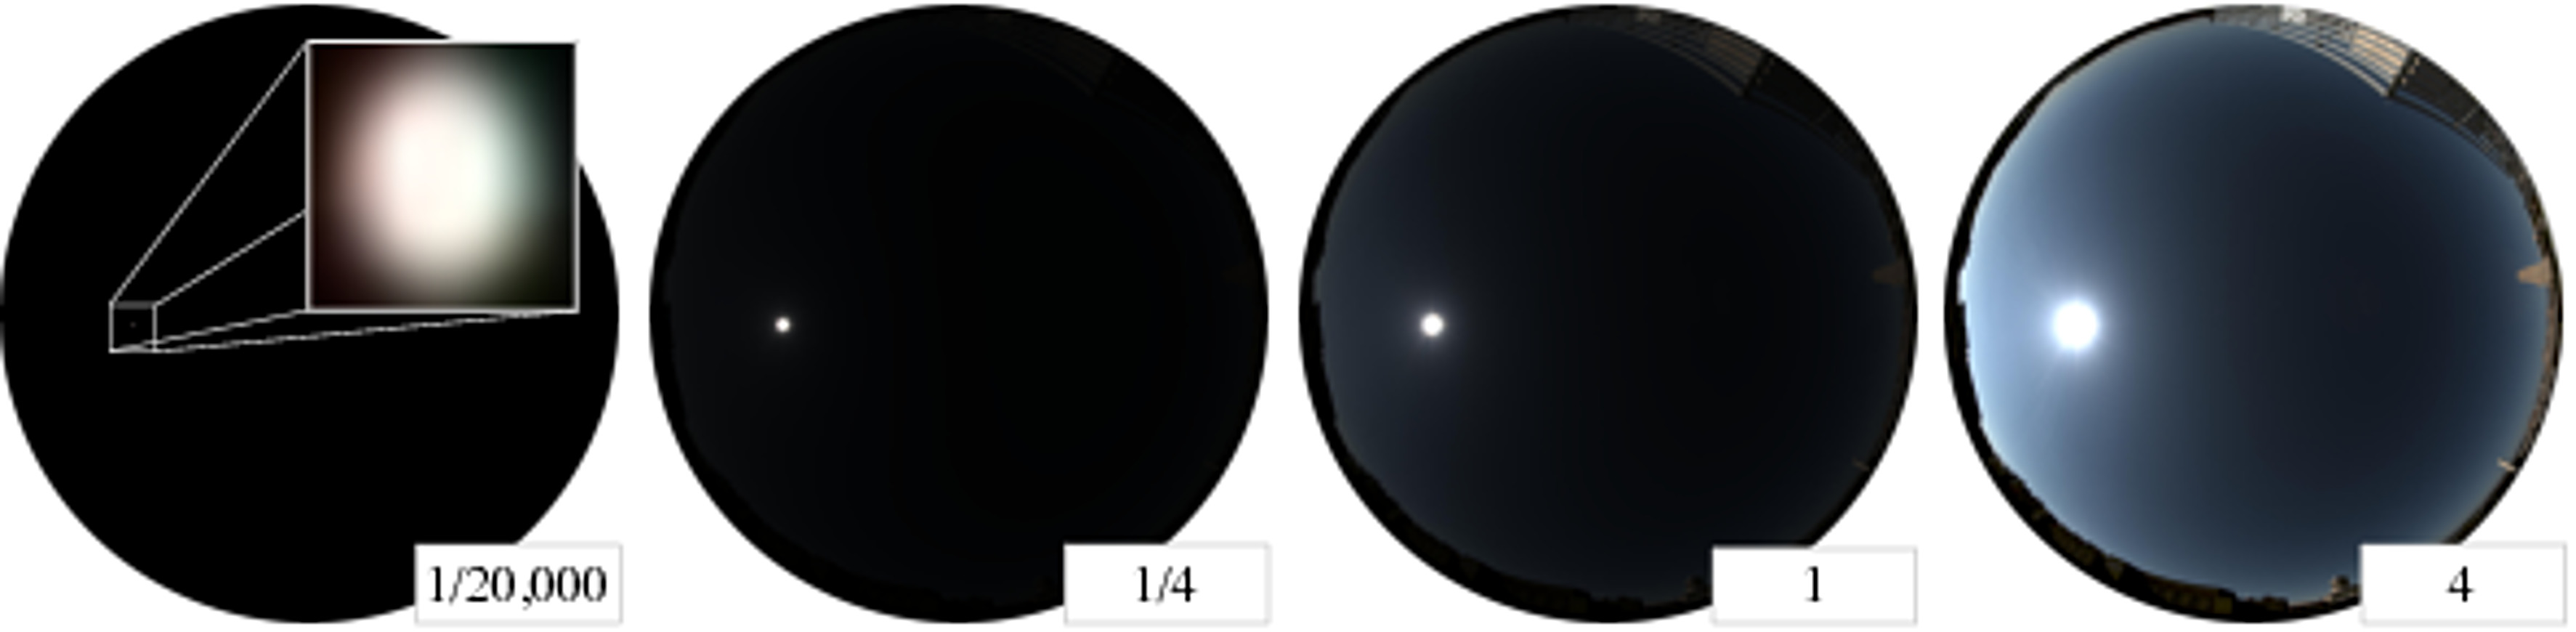
\includegraphics[width=0.96\linewidth]{exposureFig/exposureFig-row.pdf}
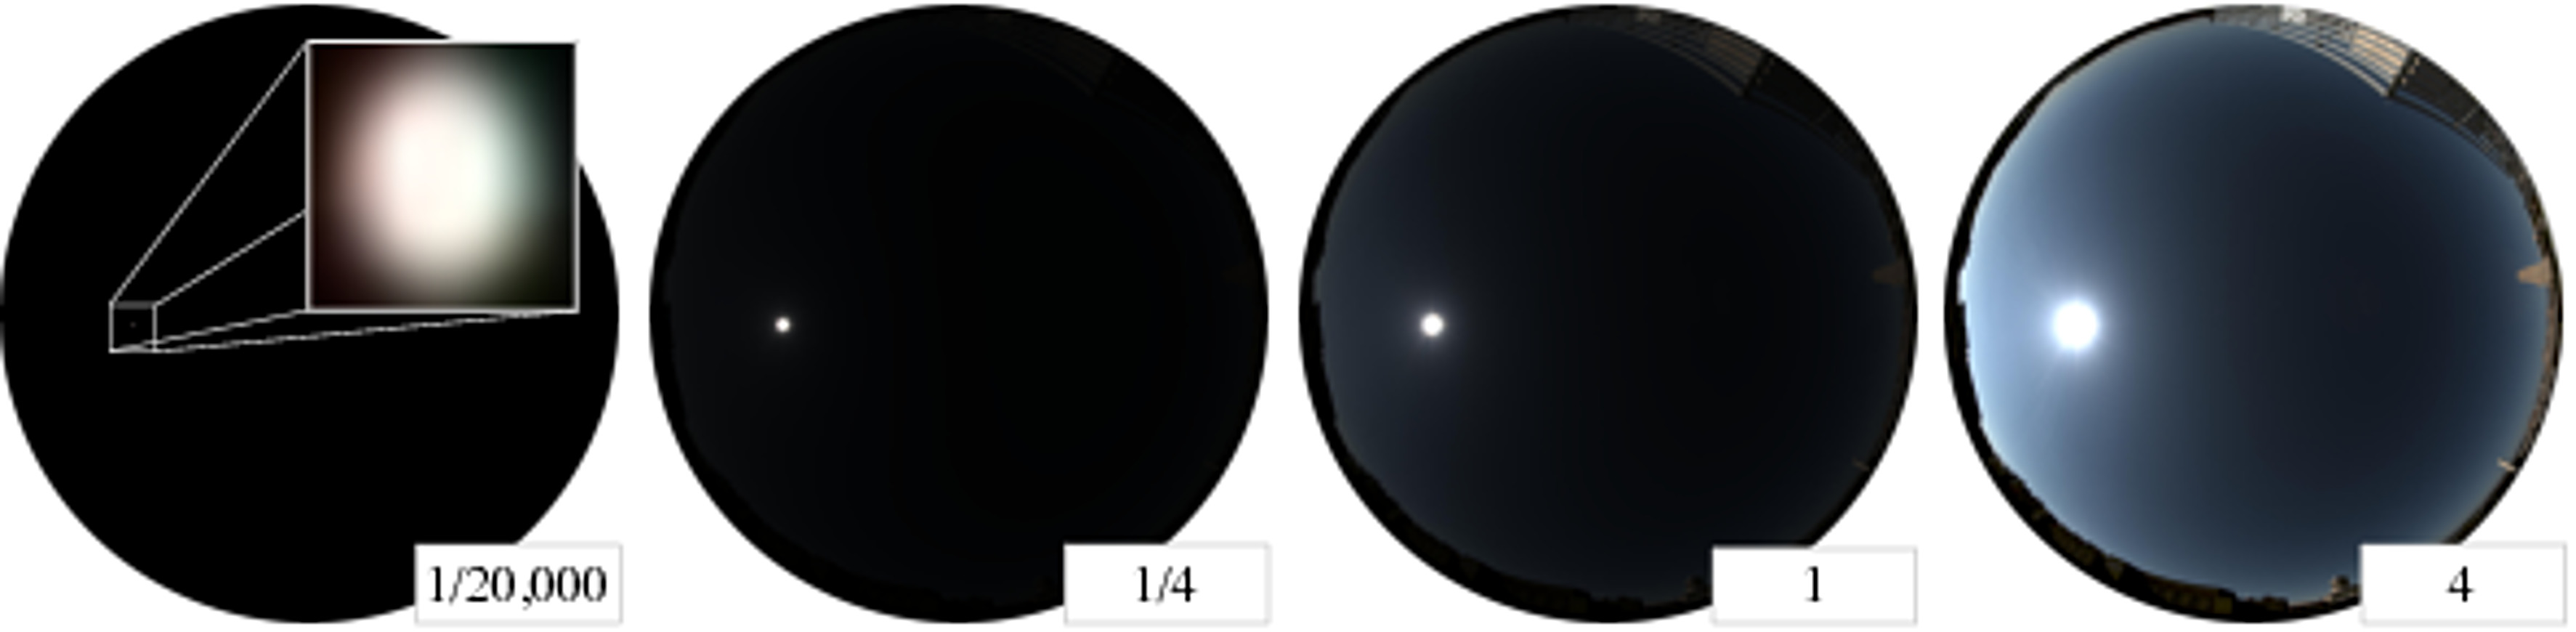
\includegraphics[width=0.96\linewidth]{exposureFig/exposureFig-row.jpg}
\caption[Sky Database]{Dynamic range in our sky database. Four different exposures of the same sky probe are shown, each expressed as factors (indicated as insets) of a reference image (1). The left-most image appears completely black, but zooming in (inset) reveals that the sun intensity is captured without saturation.}
\label{fig:exposure}
\end{figure}


\begin{figure}
\centering
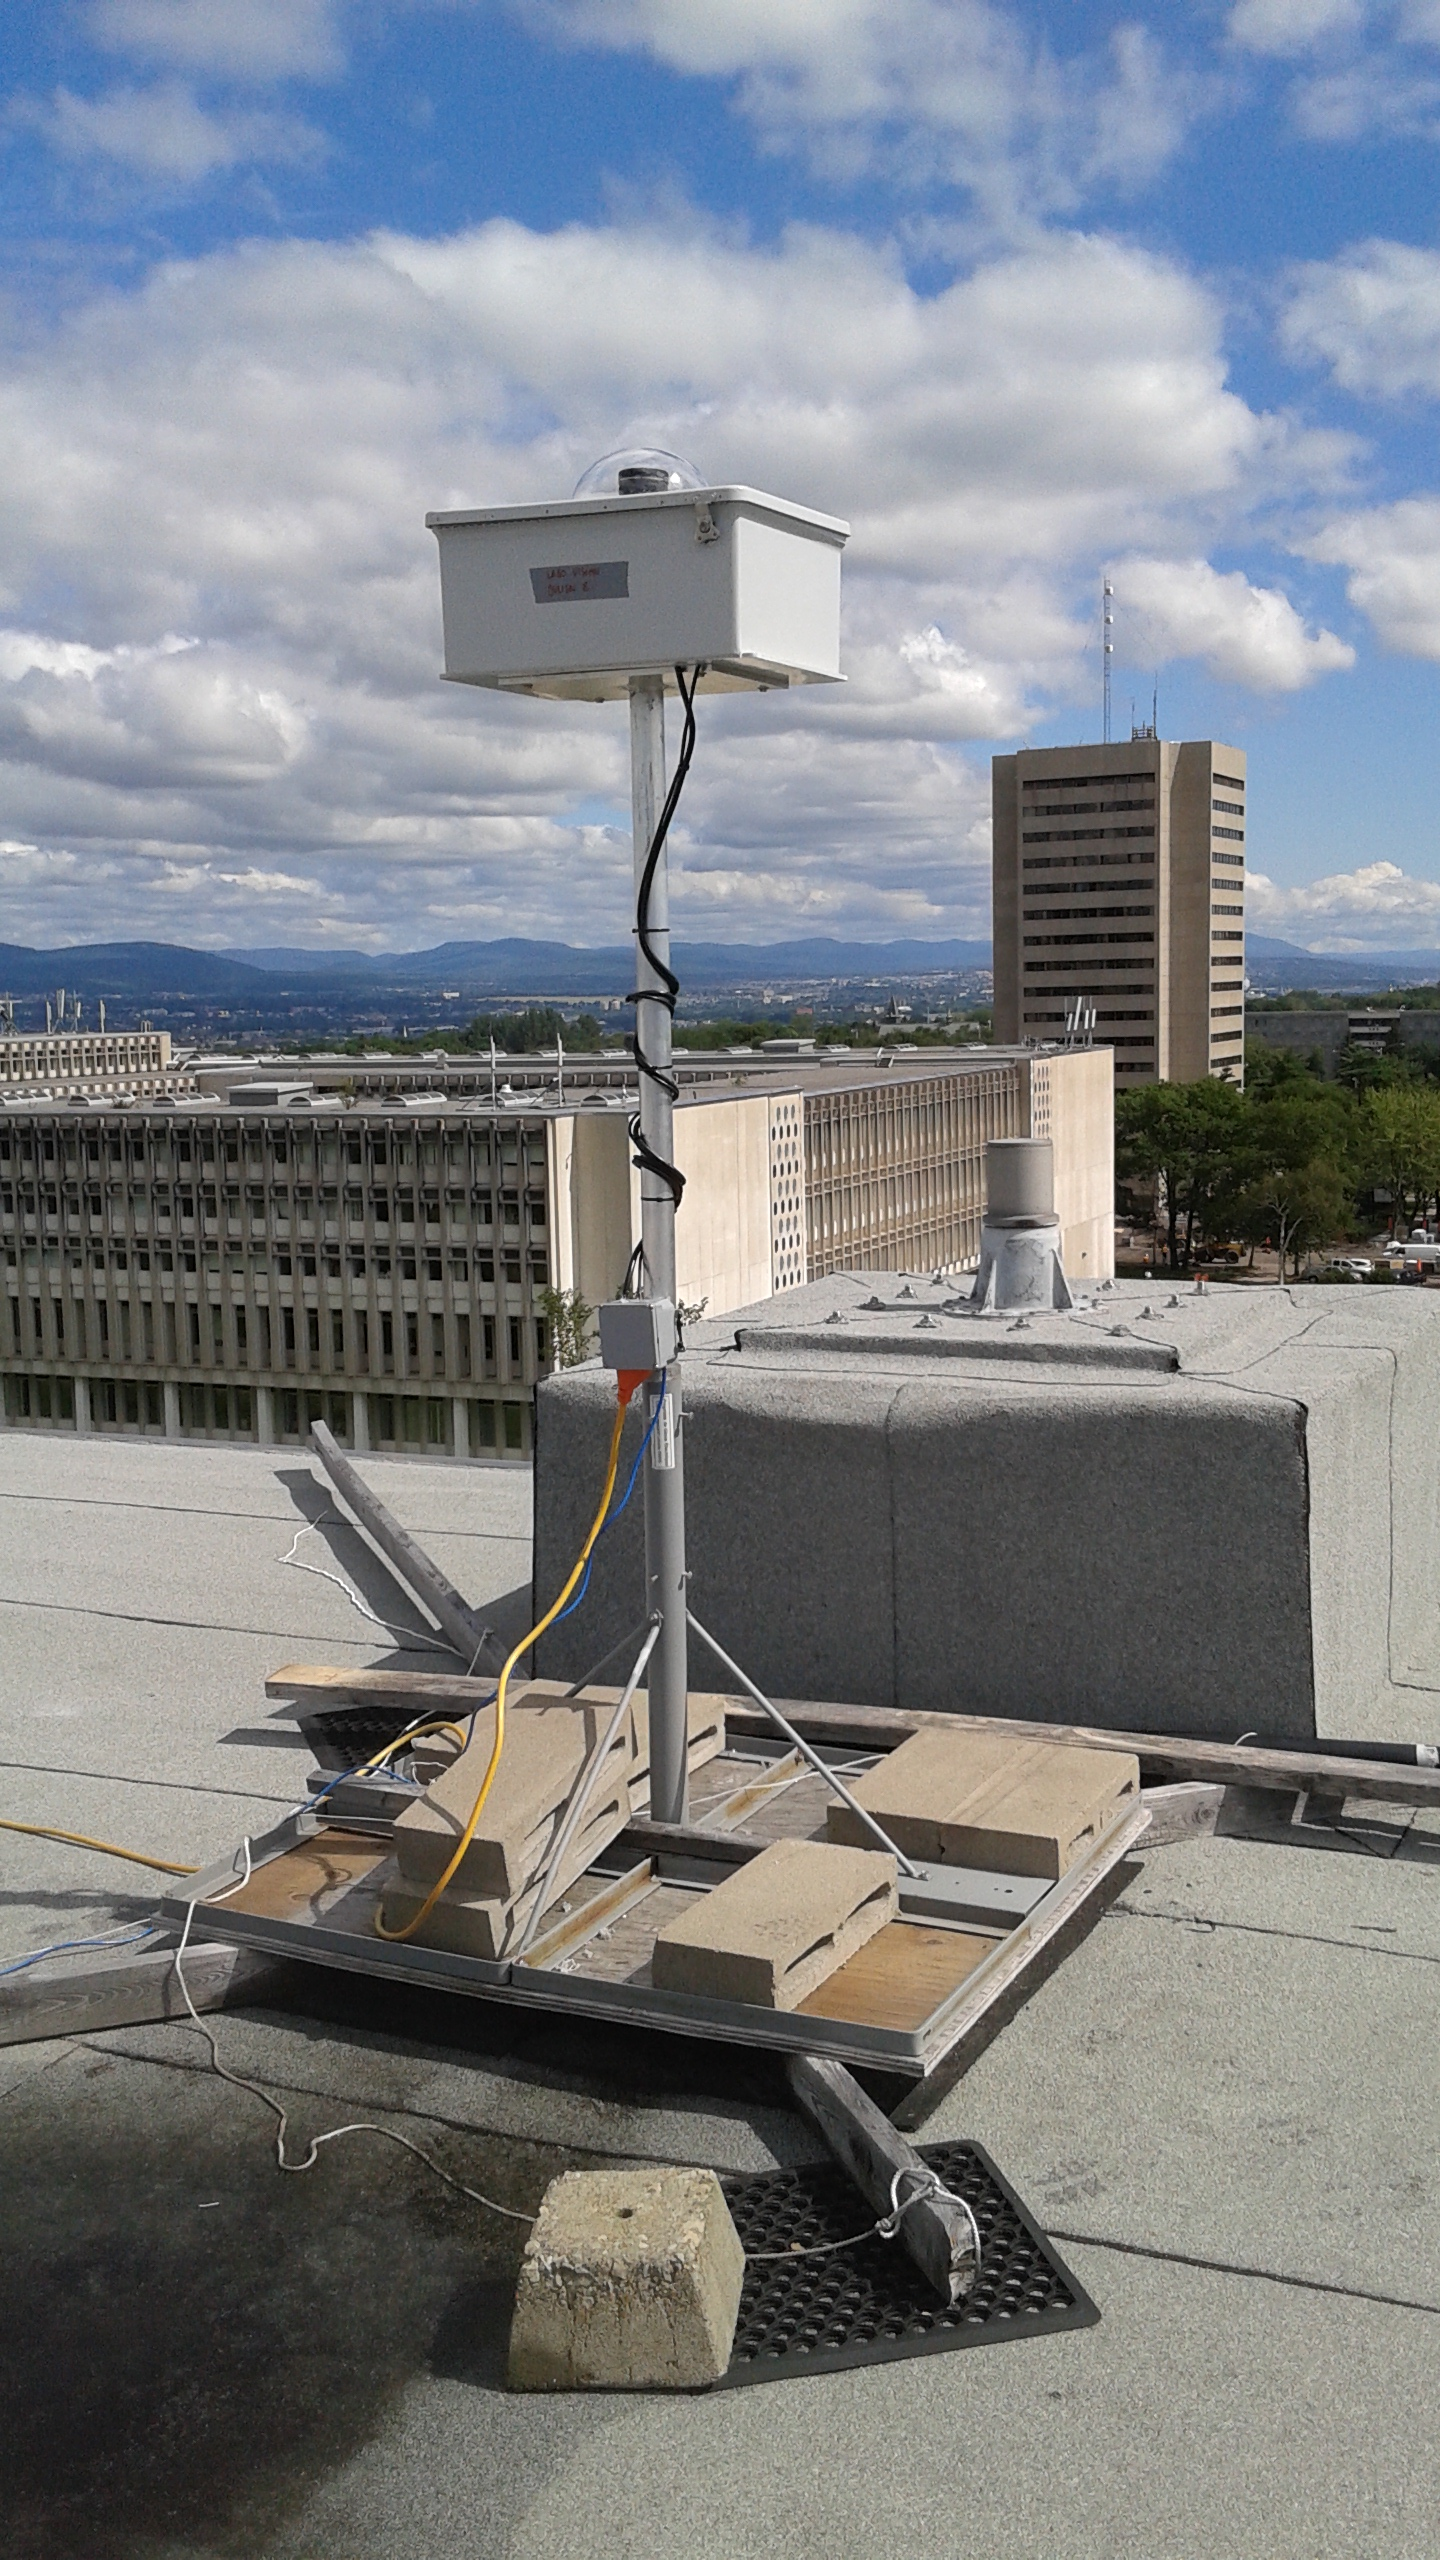
\includegraphics[width=0.45\linewidth]{database/capture_apparatus.jpg}
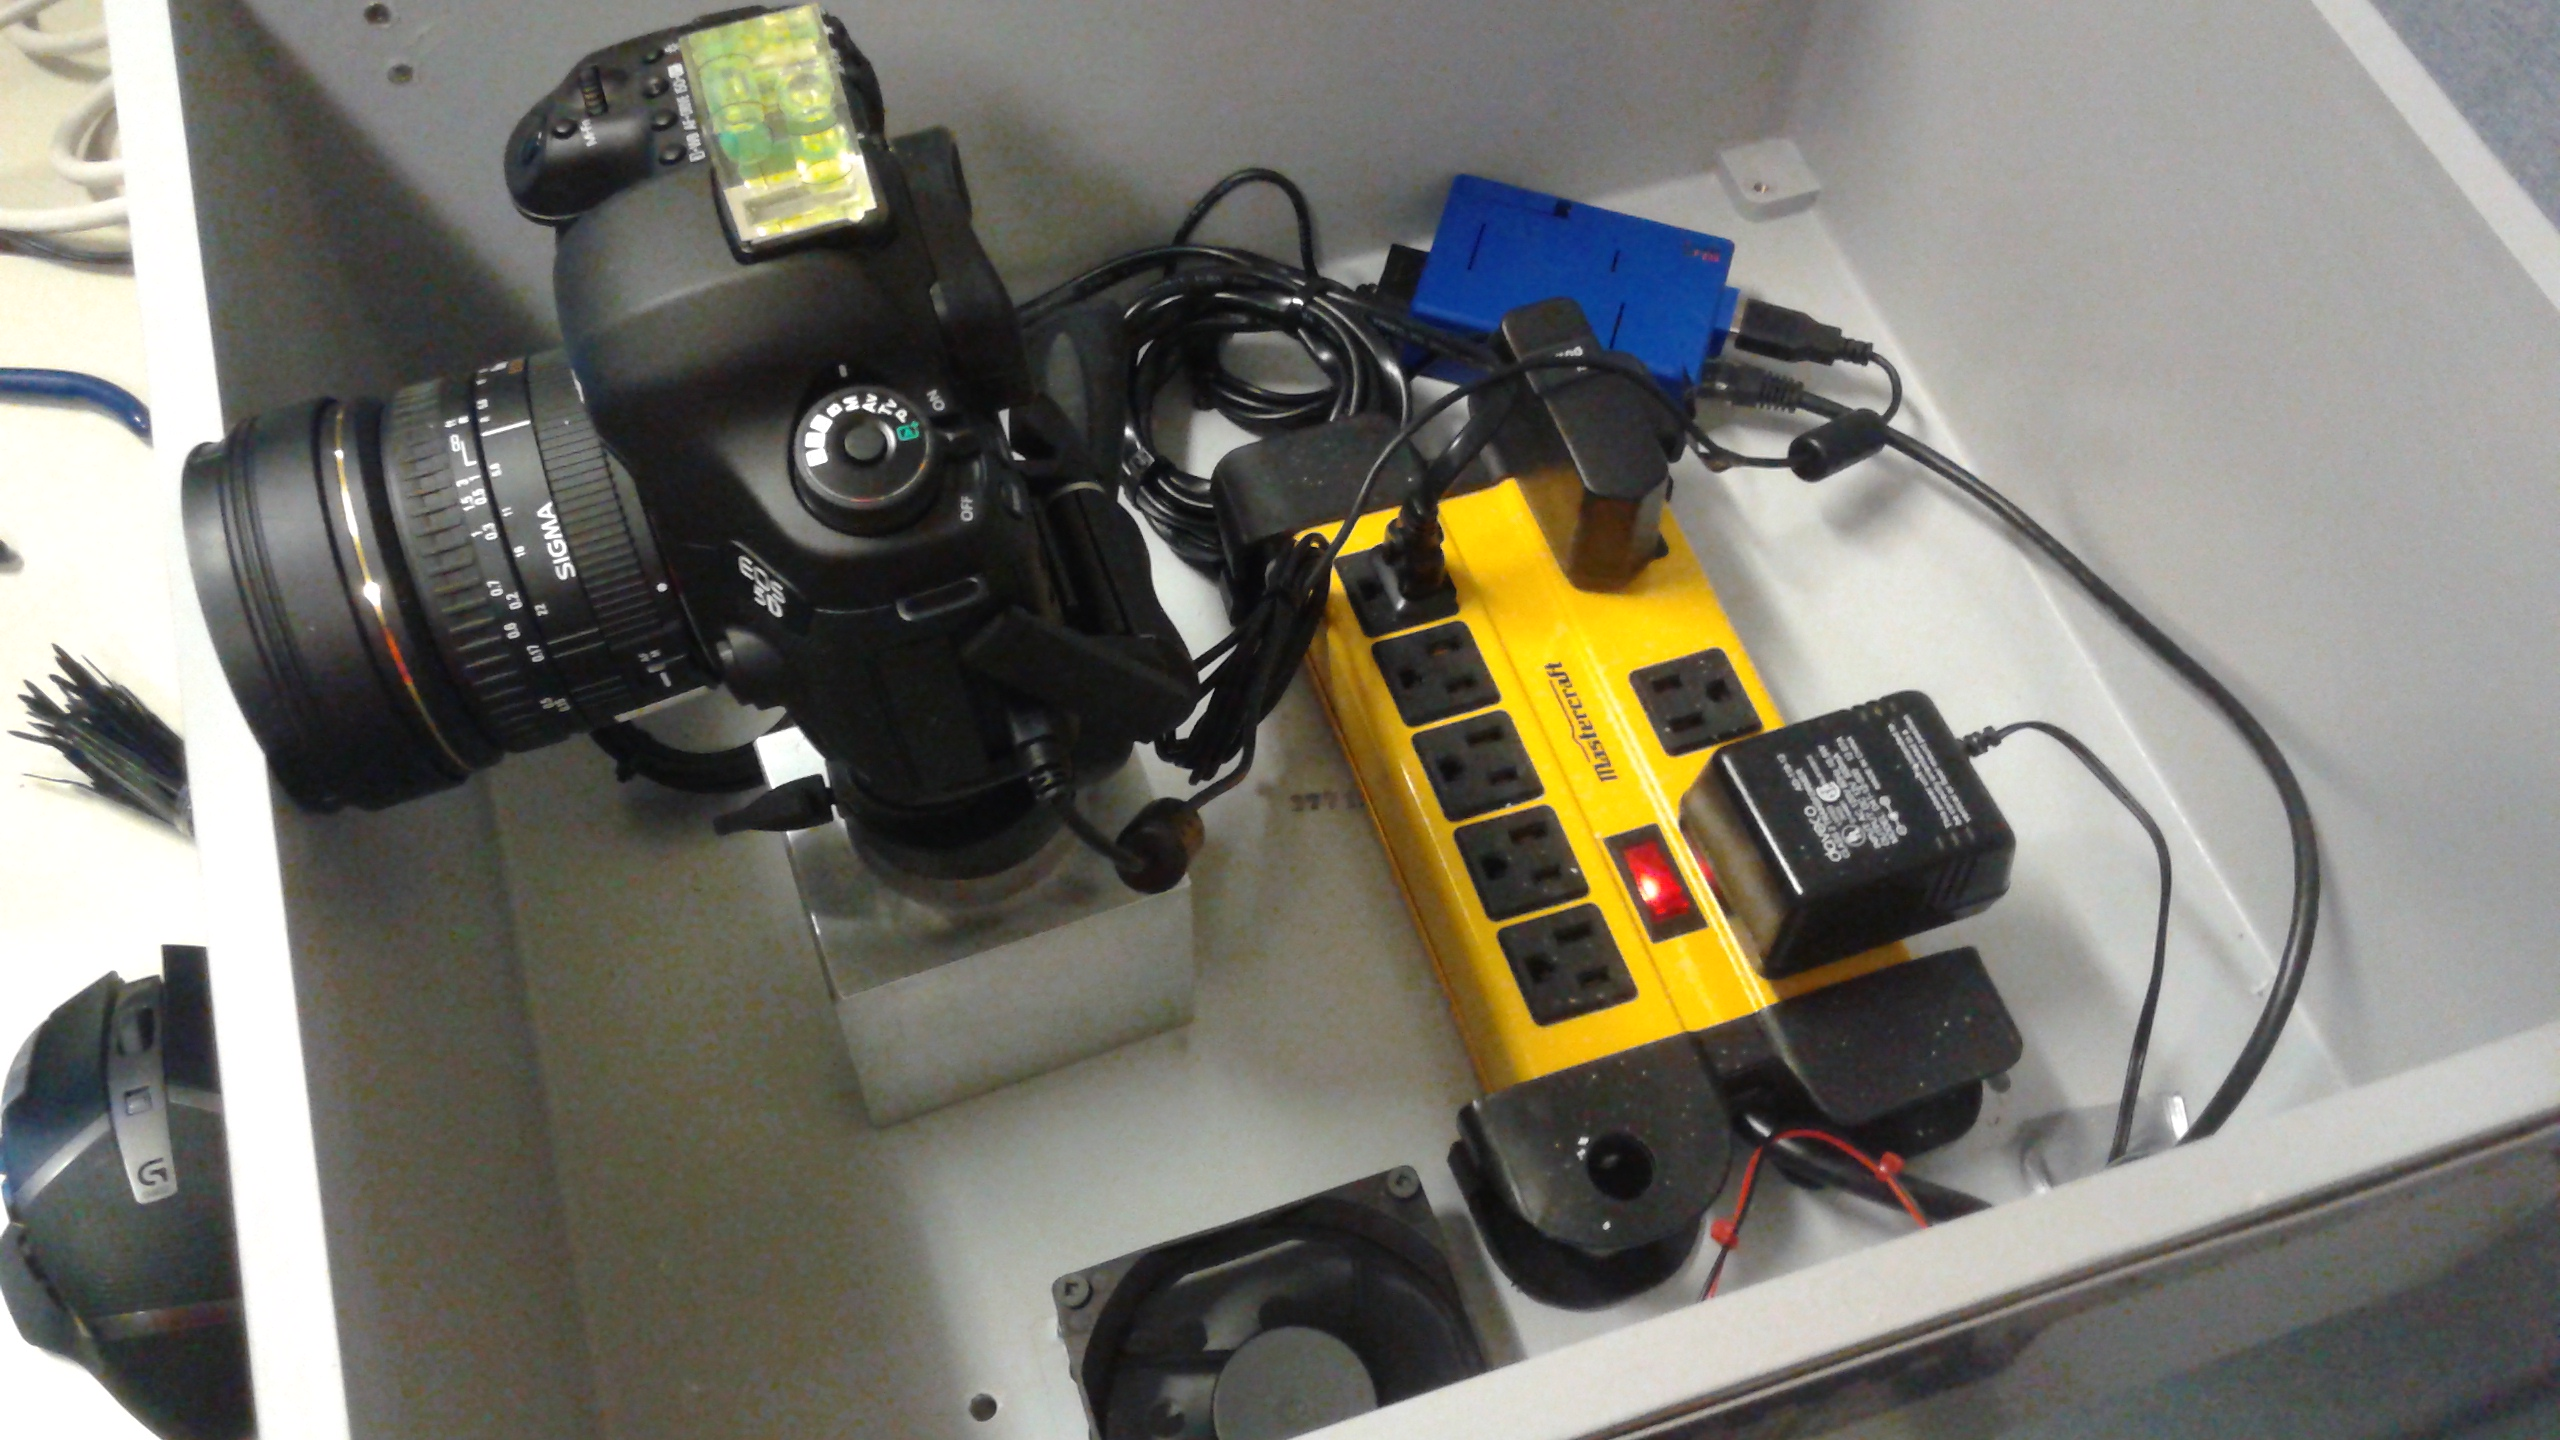
\includegraphics[width=0.45\linewidth]{database/capture_apparatus_inside.jpg}
\caption[Database capture apparatus]{Left: sky capture apparatus we developed. Right: the inside of the box, holding the Canon 5D mark III and the Raspberry Pi control system.}
\label{fig:capture-apparatus}
\end{figure}


\begin{figure}
    \centering
    \setlength{\tabcolsep}{0pt} 
    \newcommand{\customwidth}{.078\linewidth}
    \begin{tabular}{@{}rcccccccccccc@{}}
                                                     &
    \begin{minipage}{\customwidth}\centering\scriptsize 11:00 \end{minipage} &
    \begin{minipage}{\customwidth}\centering\scriptsize 11:30 \end{minipage} &
    \begin{minipage}{\customwidth}\centering\scriptsize 12:00 \end{minipage} &
    \begin{minipage}{\customwidth}\centering\scriptsize 12:30 \end{minipage} &
    \begin{minipage}{\customwidth}\centering\scriptsize 13:00 \end{minipage} &
    \begin{minipage}{\customwidth}\centering\scriptsize 13:30 \end{minipage} &
    \begin{minipage}{\customwidth}\centering\scriptsize 14:00 \end{minipage} &
    \begin{minipage}{\customwidth}\centering\scriptsize 14:30 \end{minipage} &
    \begin{minipage}{\customwidth}\centering\scriptsize 15:00 \end{minipage} &
    \begin{minipage}{\customwidth}\centering\scriptsize 15:30 \end{minipage} &
    \begin{minipage}{\customwidth}\centering\scriptsize 16:00 \end{minipage} &
    \begin{minipage}{\customwidth}\centering\scriptsize 16:30 \end{minipage}
    \\
    \begin{sideways}\begin{minipage}{\customwidth}\centering \scriptsize 08/24/2013 \\ light clouds \vspace{5pt} \end{minipage}\end{sideways} &
    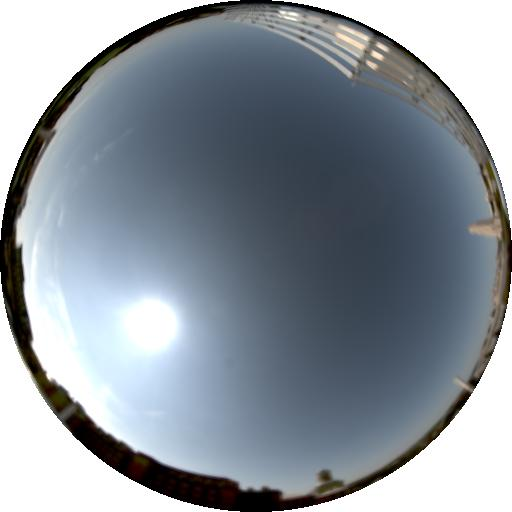
\includegraphics[width=\customwidth]{./figures/database/20130824_110040.jpg} &
    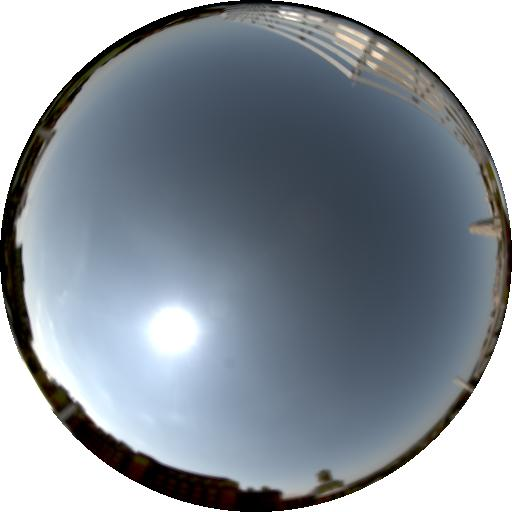
\includegraphics[width=\customwidth]{./figures/database/20130824_113038.jpg} &
    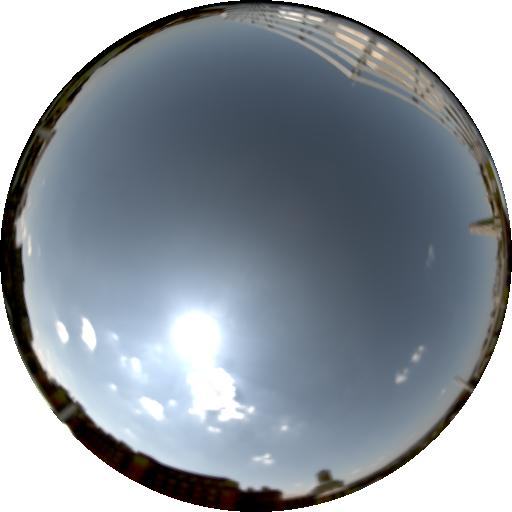
\includegraphics[width=\customwidth]{./figures/database/20130824_120033.jpg} &
    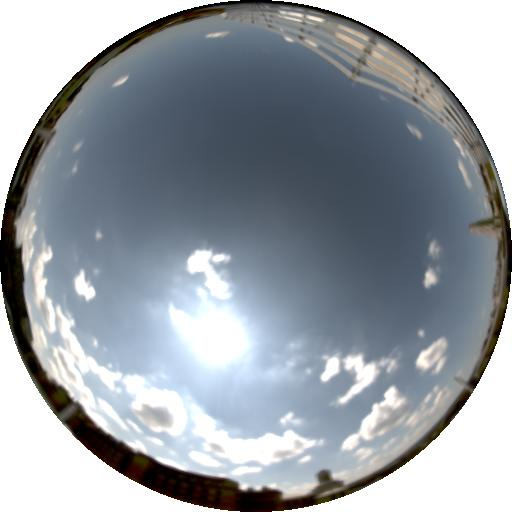
\includegraphics[width=\customwidth]{./figures/database/20130824_123024.jpg} &
    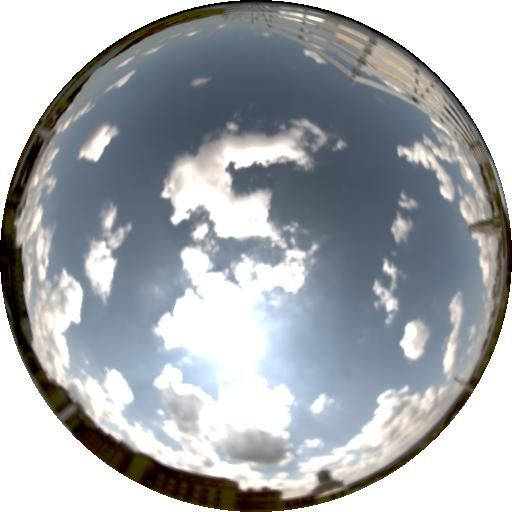
\includegraphics[width=\customwidth]{./figures/database/20130824_130014.jpg} &
    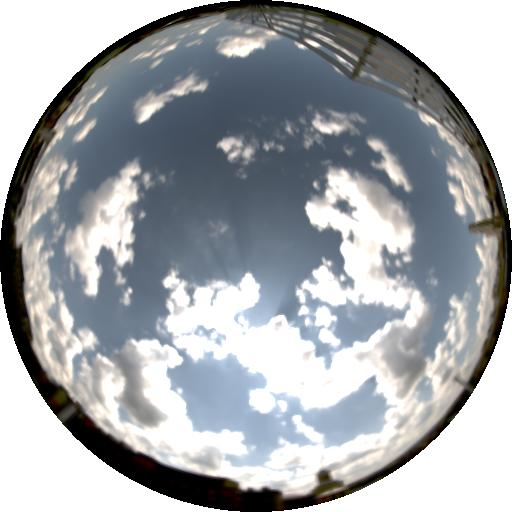
\includegraphics[width=\customwidth]{./figures/database/20130824_133006.jpg} &
    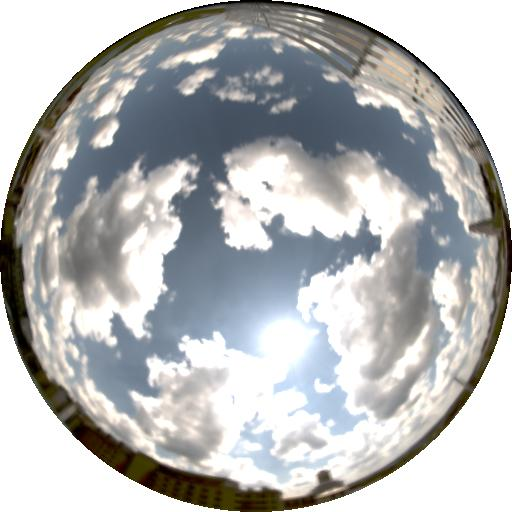
\includegraphics[width=\customwidth]{./figures/database/20130824_140002.jpg} &
    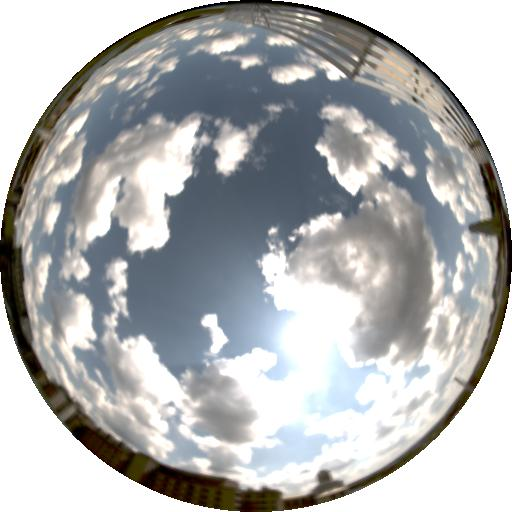
\includegraphics[width=\customwidth]{./figures/database/20130824_142960.jpg} &
    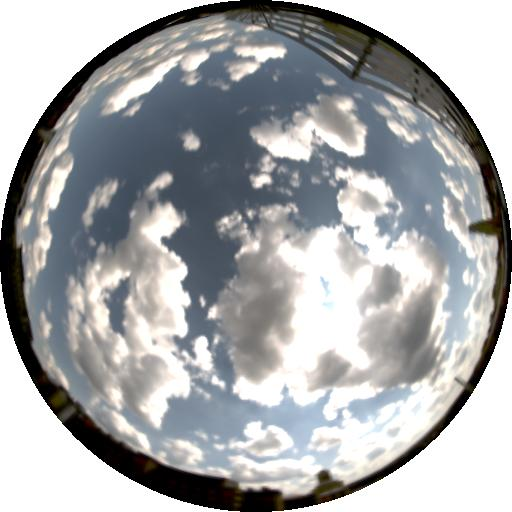
\includegraphics[width=\customwidth]{./figures/database/20130824_145957.jpg} &
    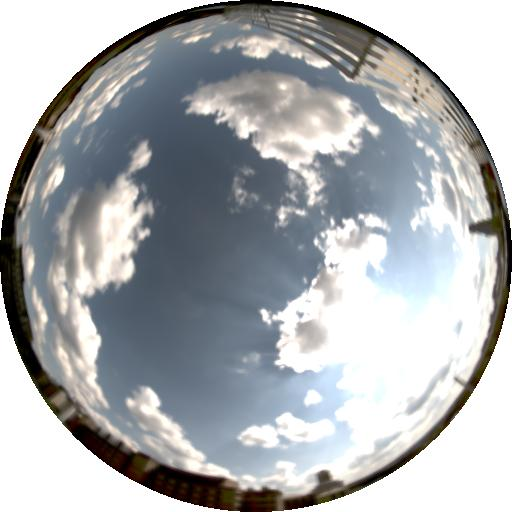
\includegraphics[width=\customwidth]{./figures/database/20130824_152946.jpg} &
    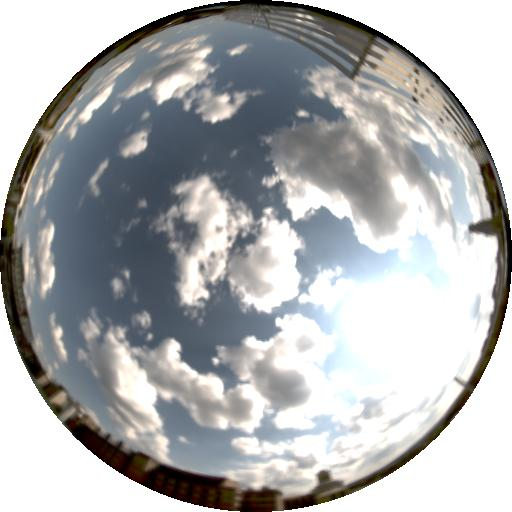
\includegraphics[width=\customwidth]{./figures/database/20130824_155938.jpg} &
    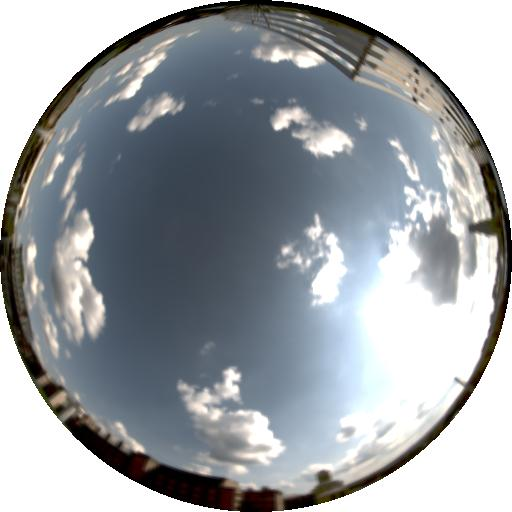
\includegraphics[width=\customwidth]{./figures/database/20130824_162933.jpg}
    \\
    \begin{sideways}\begin{minipage}{\customwidth}\centering \scriptsize 11/06/2013 \\ mixed \vspace{5pt} \end{minipage}\end{sideways} &
    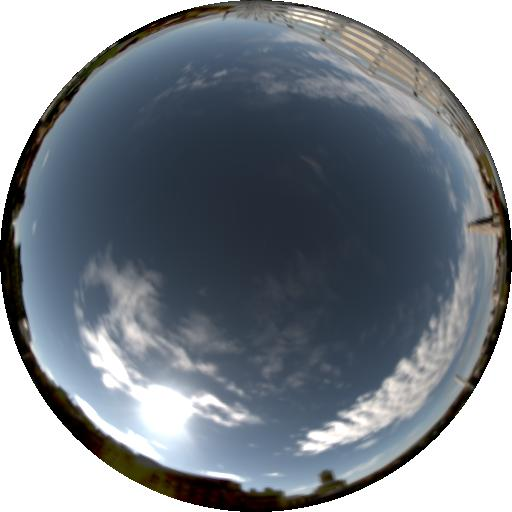
\includegraphics[width=\customwidth]{./figures/database/20131106_110951.jpg} &
    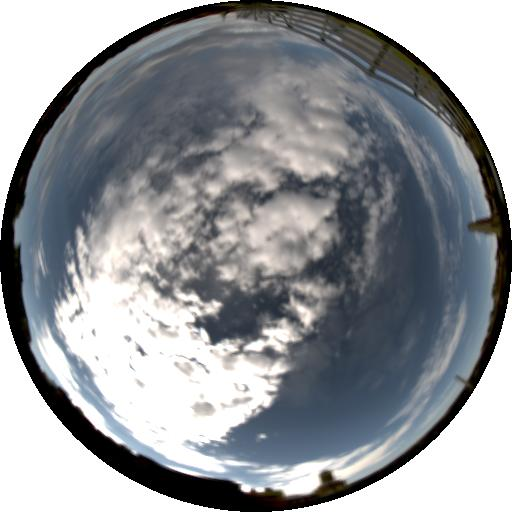
\includegraphics[width=\customwidth]{./figures/database/20131106_112948.jpg} &
    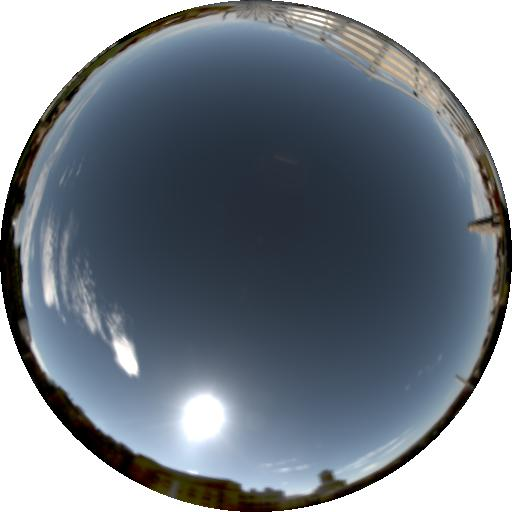
\includegraphics[width=\customwidth]{./figures/database/20131106_115943.jpg} &
    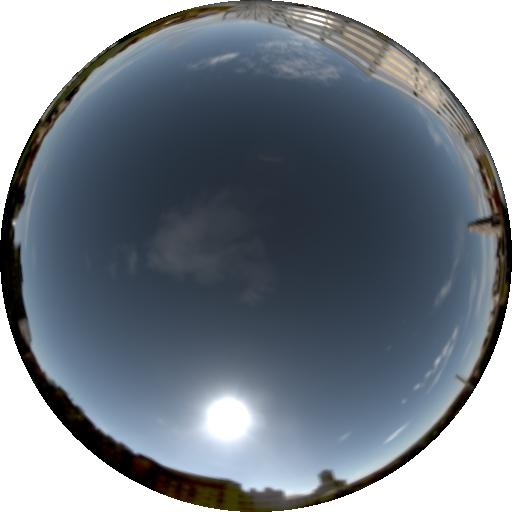
\includegraphics[width=\customwidth]{./figures/database/20131106_122939.jpg} &
    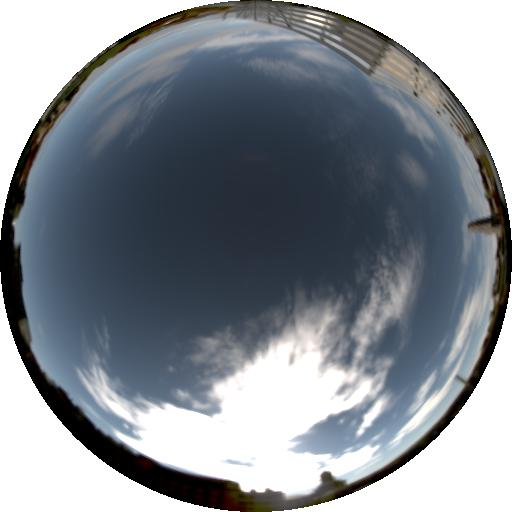
\includegraphics[width=\customwidth]{./figures/database/20131106_125937.jpg} &
    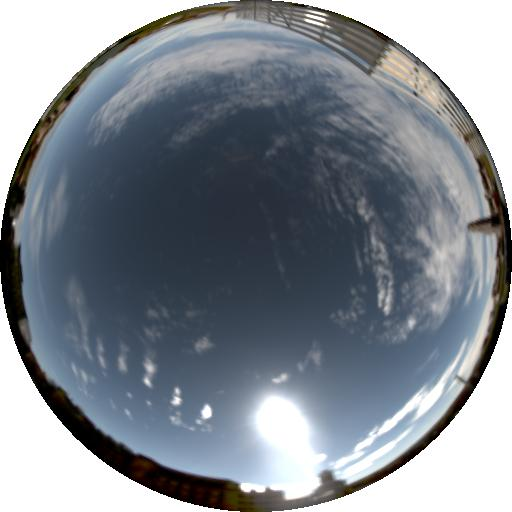
\includegraphics[width=\customwidth]{./figures/database/20131106_132936.jpg} &
    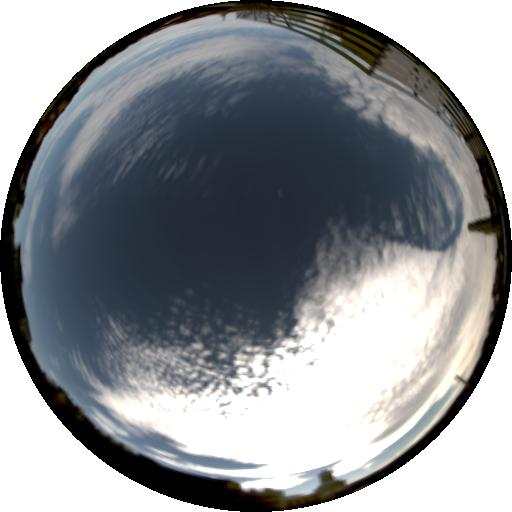
\includegraphics[width=\customwidth]{./figures/database/20131106_135932.jpg} &
    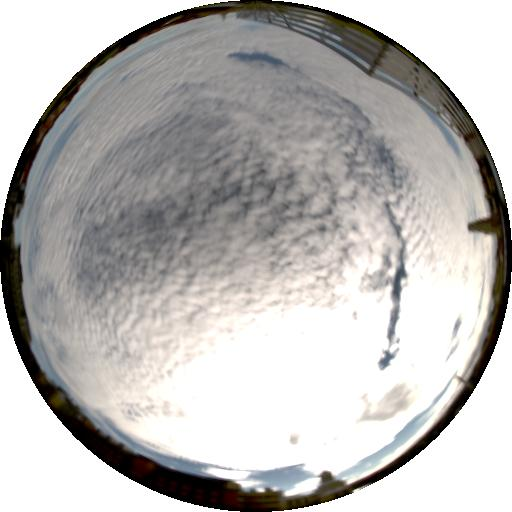
\includegraphics[width=\customwidth]{./figures/database/20131106_142922.jpg} &
    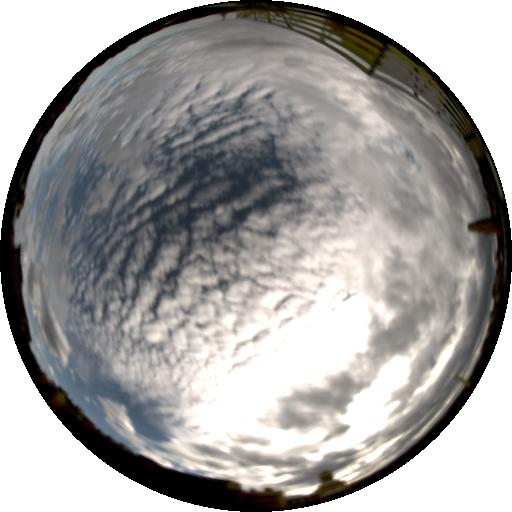
\includegraphics[width=\customwidth]{./figures/database/20131106_145915.jpg} &
    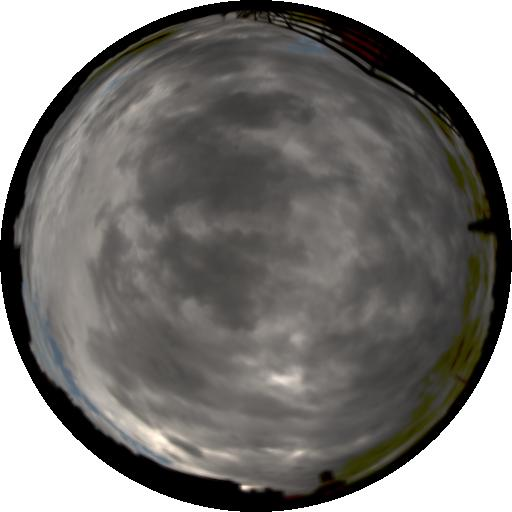
\includegraphics[width=\customwidth]{./figures/database/20131106_152913.jpg} &
    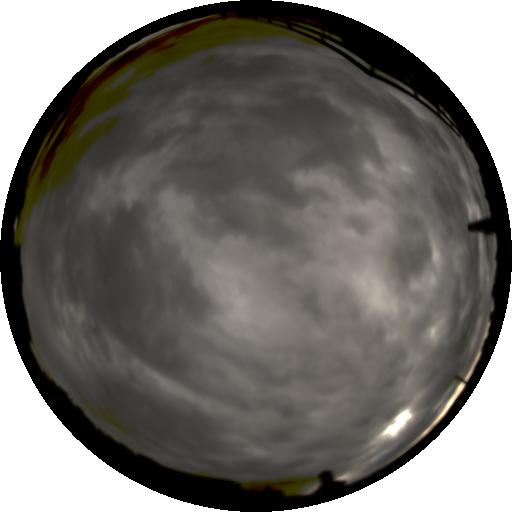
\includegraphics[width=\customwidth]{./figures/database/20131106_155906.jpg} &
    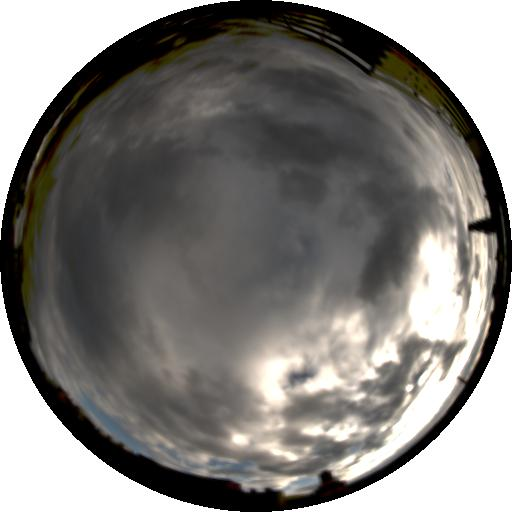
\includegraphics[width=\customwidth]{./figures/database/20131106_163057.jpg}
    \\
    \begin{sideways}\begin{minipage}{\customwidth}\centering \scriptsize 11/08/2014 \\ heavy clds.\vspace{5pt} \end{minipage}\end{sideways} &
    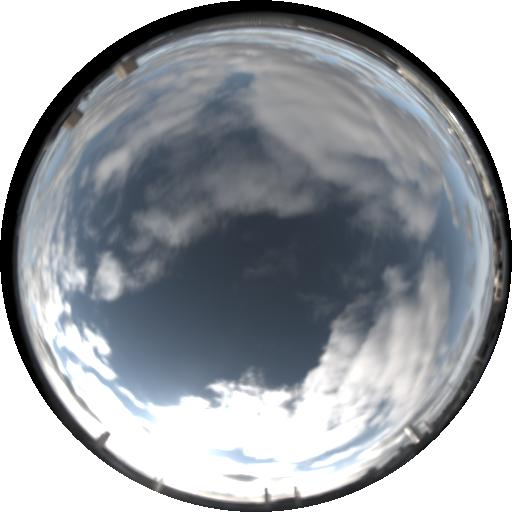
\includegraphics[width=\customwidth]{./figures/database/20141108_110025.jpg} &
    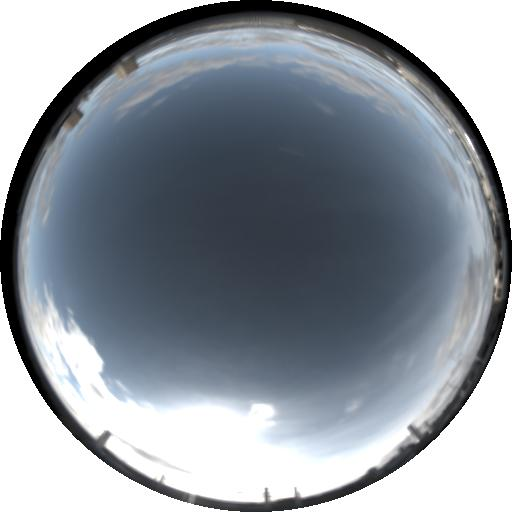
\includegraphics[width=\customwidth]{./figures/database/20141108_113025.jpg} &
    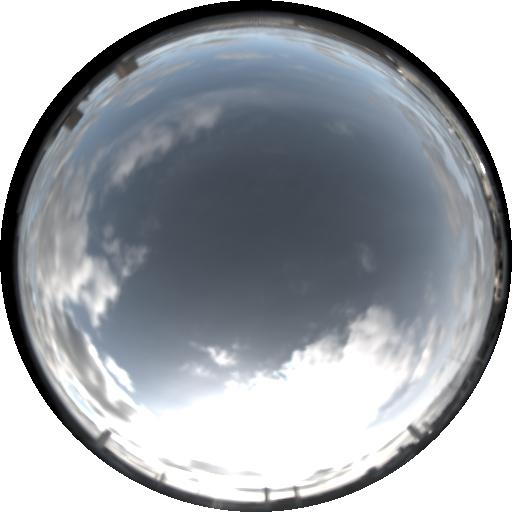
\includegraphics[width=\customwidth]{./figures/database/20141108_120025.jpg} &
    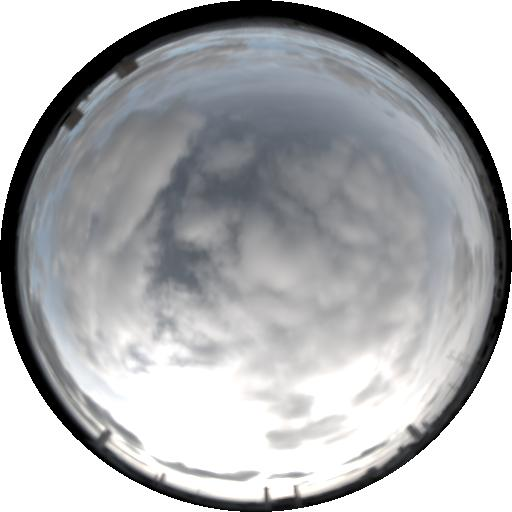
\includegraphics[width=\customwidth]{./figures/database/20141108_123025.jpg} &
    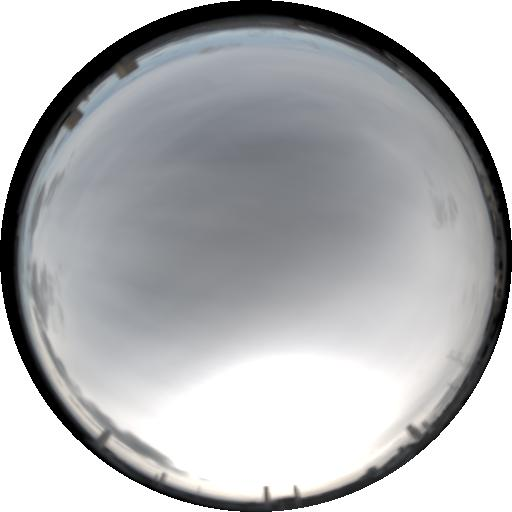
\includegraphics[width=\customwidth]{./figures/database/20141108_130025.jpg} &
    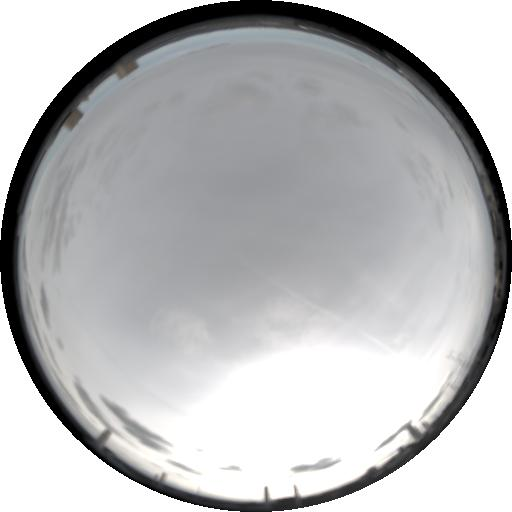
\includegraphics[width=\customwidth]{./figures/database/20141108_133025.jpg} &
    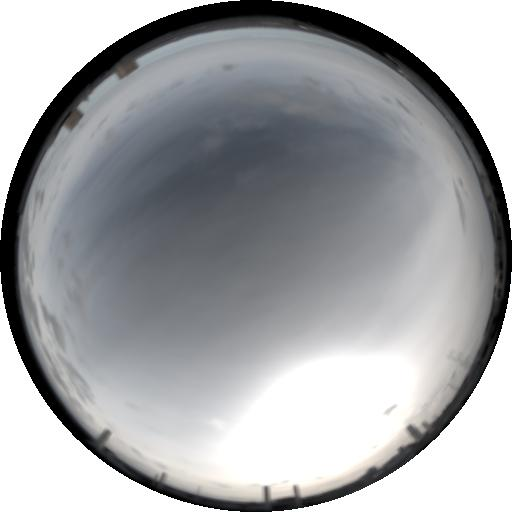
\includegraphics[width=\customwidth]{./figures/database/20141108_140025.jpg} &
    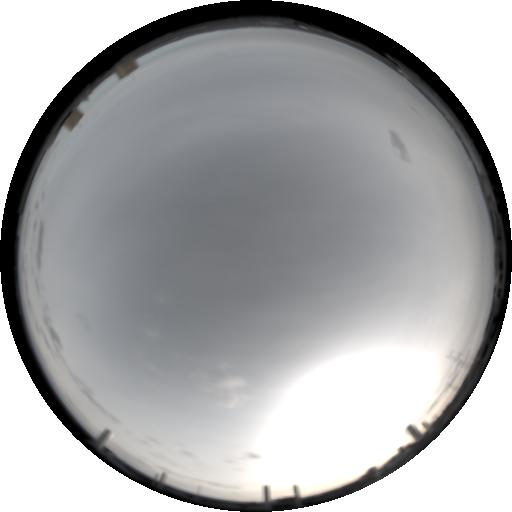
\includegraphics[width=\customwidth]{./figures/database/20141108_143025.jpg} &
    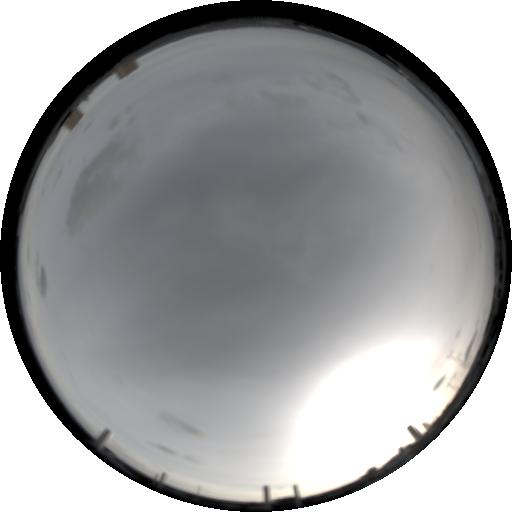
\includegraphics[width=\customwidth]{./figures/database/20141108_150025.jpg} &
    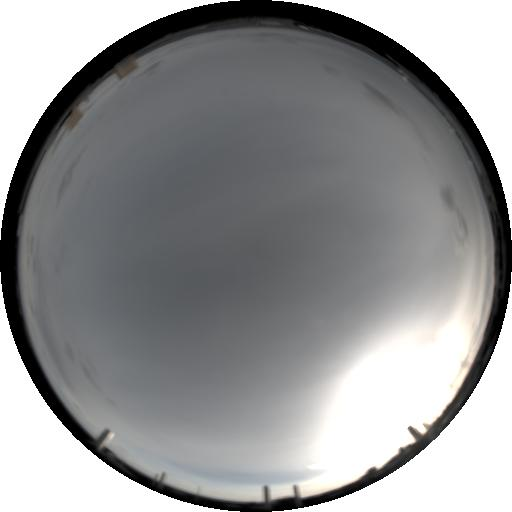
\includegraphics[width=\customwidth]{./figures/database/20141108_153025.jpg} &
    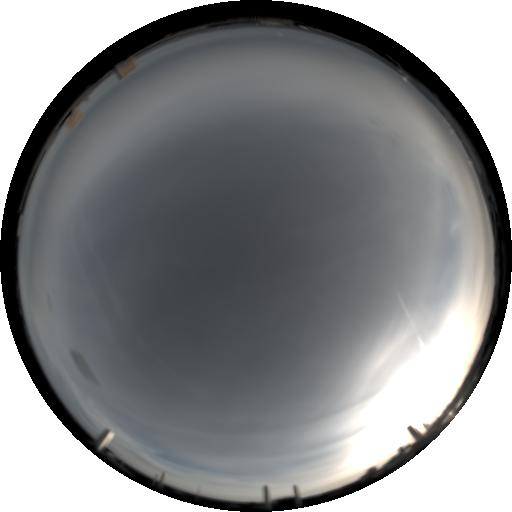
\includegraphics[width=\customwidth]{./figures/database/20141108_160025.jpg} &
    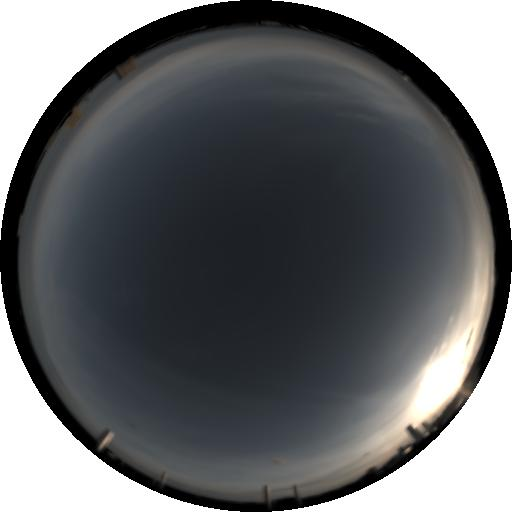
\includegraphics[width=\customwidth]{./figures/database/20141108_163025.jpg}

    \\

    \end{tabular}
    \caption[HDRDB dataset excerpt]{Examples from our dataset of HDR outdoor illumination conditions. In all, our dataset contains 3,800 different illumination conditions, captured from 10{:}30 until 16{:}30, during 23 days, spread over ten months and at two geographical locations. Each image is stored in the 32-bit floating point EXR format, and shown tone mapped here for display (with $\gamma = 1.6$). The companion video\footnote{Available at \url{http://vision.gel.ulaval.ca/~jflalonde/projects/outdoorPS/index.html}} shows time-lapse sequences for these sky environment maps.}
    \label{fig:database}
\end{figure}


\section{Image formation model}
\label{iccp15:ifm}

Consider a small, Lambertian surface patch with normal vector ${\bf n}$ and albedo $\rho$ (w.l.o.g., assume albedo is monochromatic). At time $t$, this surface patch is observed under natural, outdoor illumination represented by the environment map $L_t(\boldomega)$ (\eg, fig.~\ref{fig:database}), with $\boldomega$ denoting a direction in the unit sphere. With an orthographic camera model, this patch is depicted as an image pixel with intensity
%
\begin{equation}
    b_t = \frac{\rho}{\pi} \int_{\Omega_{\bf n}} L_t(\mathbf{\boldomega}) \langle \boldomega, {\bf n} \rangle d\omega \,,
    \label{eqn:imageformation-continuous}
\end{equation}
%
where $\langle \cdot, \cdot \rangle$ denotes the dot product. Integration is carried out over the hemisphere of incoming light, $\Omega_{\bf n}$, defined by the local orientation ${\bf n}$ of the surface, fig.~\ref{fig:normal-diagram}. This hemisphere corresponds to an occlusion (or attached shadow) mask; only half of the pixels in the environment map contribute to the illumination of the surface patch. To make the analysis tractable and independent on object geometry, this chapter focuses on the simpler case without cast shadows.

\begin{figure}
    \centering
    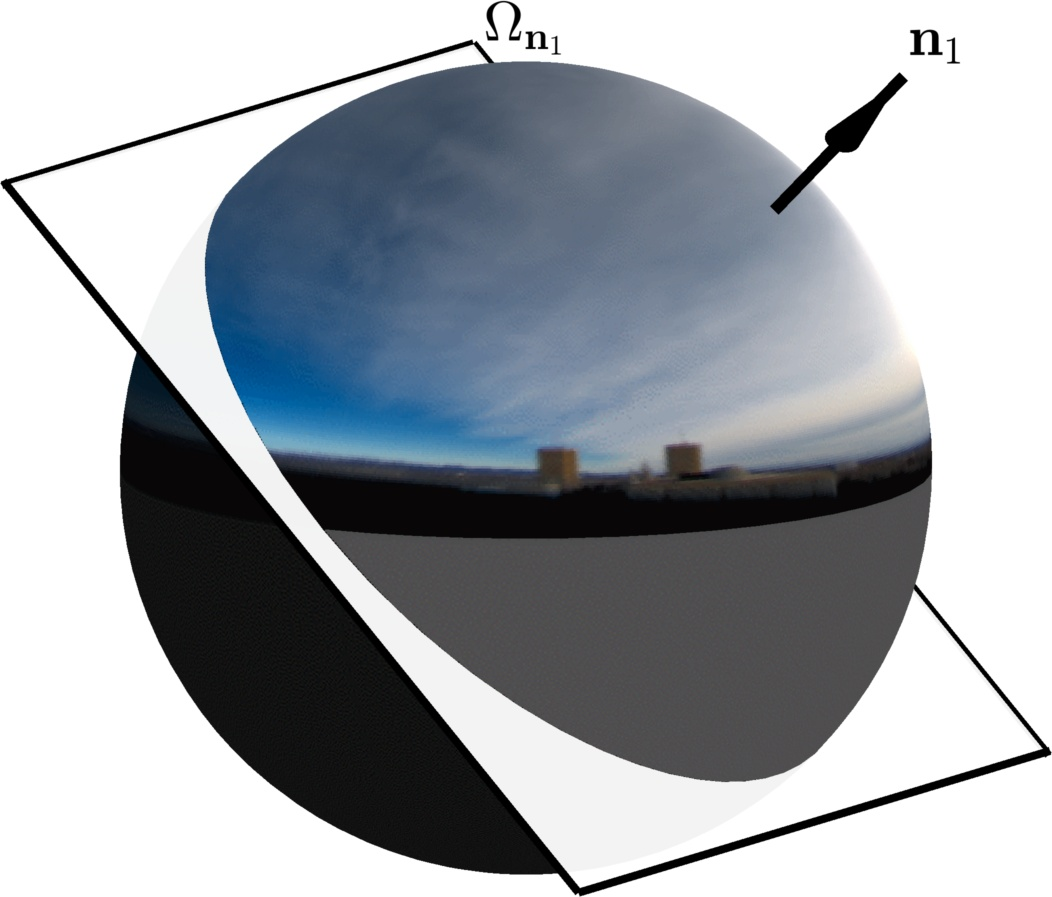
\includegraphics[width=.495\linewidth]{./figures/diagramFig/diagram1.jpg}
    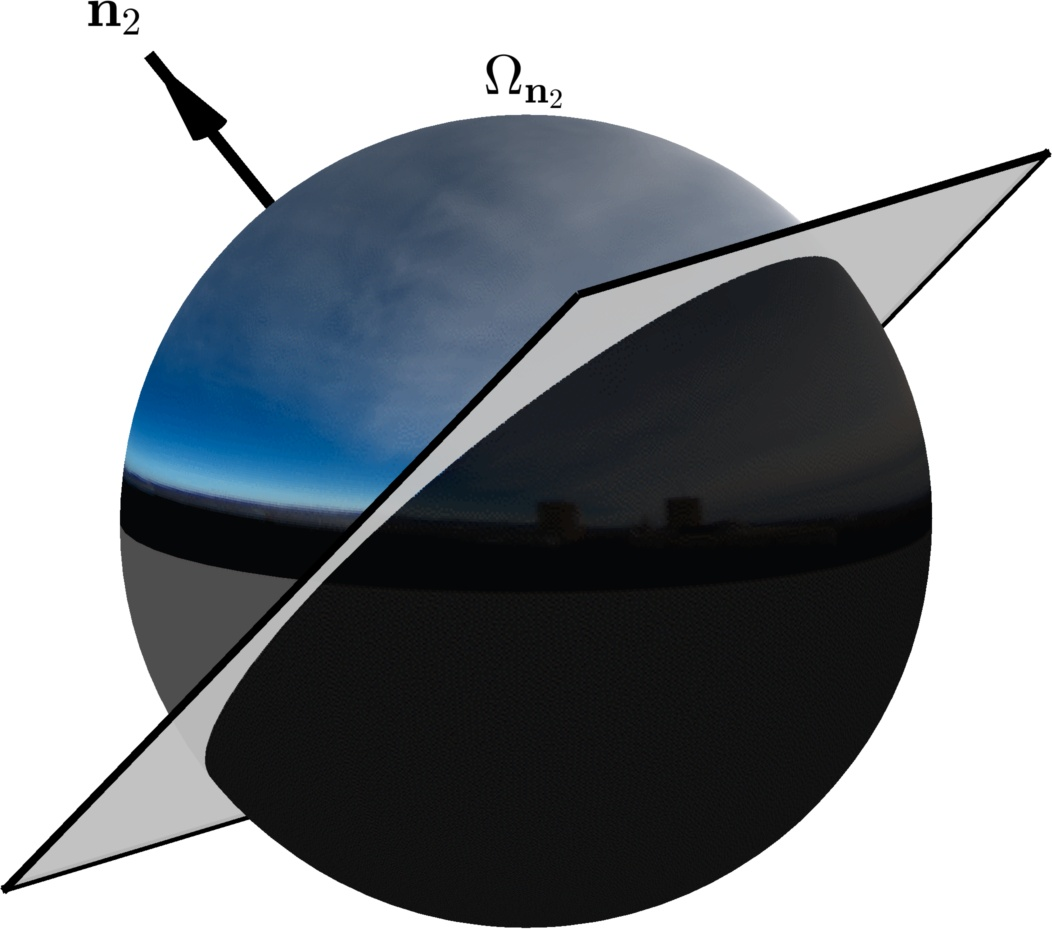
\includegraphics[width=.495\linewidth]{./figures/diagramFig/diagram2.jpg}
    \caption[Hemispheres defined by surface normals]{A normal $\mathbf{n}$ defines an integration domain $\Omega_{\mathbf{n}}$ equivalent to a hemisphere on the entire spherical environment map. Only light emanating from this hemisphere contribute to the shading on that patch. Therefore, patches with different normals are lit differently even if the environment map is the same.}
    \label{fig:normal-diagram}
\end{figure}

This image formation model is then discretized as,
%
\begin{equation}
b_t = \frac{\rho}{\pi}\sum_{\boldomega_j \in \Omega_{\bf n}} \widehat{L}_t(\boldomega_j) \langle \boldomega_j, {\bf n} \rangle\,,
\label{eqn:imageformation-discrete}
\end{equation}
%
with $\widehat{L}_t(\boldomega_j) = L_t(\boldomega_j)\Delta\omega_j$ representing the environment map weighted by the solid angle $\Delta\omega_j$ spanned by pixel $j$ ($\Delta\omega_j$, $\forall j$, are normalized as to sum to $2\pi$). Eq.~$\eqref{eqn:imageformation-discrete}$ can be further summarized into the equivalent form
%
\begin{equation}
b_t = {\bf \bar l}_t^T \mathbf{x}
\label{eqn:imageformation-simplified}
\end{equation}
where ${\bf x} = \rho {\bf n}$ is the albedo-scaled normal vector and
\begin{equation}
{\bf \bar l}_t = \frac{1}{\pi} \sum_{\boldomega_j \in \Omega_{\bf n}} \widehat{L}_t(\boldomega_j) \boldomega_j \in \mathbb{R}^3
\label{eqn:mean-light}
\end{equation}
is interpreted as the {\em mean light vector} for the environment map at a time $t$. It is important to note that, as opposed to the traditional PS scenario where point light sources are fixed and thus independent of ${\bf n}$, here the {\em per-pixel} MLV is a function of $\mathbf{n}$. Thus, patches with different orientations define different sets of MLVs (as discussed later and shown in fig.~\ref{fig:realShiftNormal}).

Given multiple images taken at times $t \in \{1,2,\ldots,T\}$, we collect all photometric constraints for patch ${\bf x}$ to obtain:
\begin{equation}
\mathbf{b} =
\begin{bmatrix}
 b_1 \\ b_2 \\ \vdots \\ b_T
\end{bmatrix}
=
\begin{bmatrix}
 {\bf \bar l}_1^T \\ {\bf \bar l}_2^T \\ \vdots \\ {\bf \bar l}_T^T
\end{bmatrix}
{\bf x} = \mathbf{L} \mathbf{x} \,.
\label{eqn:matrix-form}
\end{equation}
With~\eqref{eqn:matrix-form}, this model of natural environmental illumination becomes quite similar to a model with a distant point light source, the well-known case in PS. However, note that each ${\bf \bar l}_t$ in ${\bf L}$ is a function of $\Omega_{\bf n}$ and, thus, of ${\bf n}$.

Most importantly, in outdoor PS, a well-defined solution ${\bf x}$ may exist even if the relative sun motion is nearly planar during a certain time interval. Instead of relying solely on sun direction, now, the solution requires non-coplanar mean light vectors ${\bf \bar l}_t$, which are determined by a comprehensive set of natural illumination factors.

\section{Modeling uncertainty}
\label{sec:modeling_uncertainty}

From~\eqref{eqn:matrix-form}, the least-squares solution ${\bf x} = ({\bf L}^T{\bf L})^{-1}{\bf L}^T{\bf b}$ of outdoor PS is clearly affected by the condition number of ${\bf L}$. Thus, we next characterize how well the solution ${\bf x}$ is constrained by natural, outdoor illumination within a given time interval (\eg, one day)---which is encoded by the set of mean light vectors ${\bf \bar l}_t$ in ${\bf L}$ or, equivalently, the set of environment maps $L_t(\cdot)$.

To assess the reliability of a solution ${\bf x}$, we follow standard practice in PS~\cite{klaudiny-prl-14,sun-ivc-07} and consider image measurements corrupted by zero-mean Gaussian noise with equal variance $\sigma^2$ (as least squares estimation is only optimal for this practical, most common noise model). Thus, ${\bf b}$ in~\eqref{eqn:matrix-form} follows a normal distribution:
%
\begin{equation}
{\bf b} \sim \mathcal{N}\left( \boldmu_b, \sigma^2 {\bf I} \right)\,,
\end{equation}
%
where $\boldmu_b$ has the (unknown) uncorrupted pixel values.

Since the desired least-squares solution for the albedo-scaled normal, ${\bf x} = \left({\bf L}^T{\bf L}\right)^{-1}{\bf L}^T{\bf b}$, is a linear transformation of a Gaussian random vector, it is easy to show that
%
\begin{equation}
{\bf x} \sim \mathcal{N} \left( \boldmu_x, \sigma^2({\bf L}^T{\bf L})^{-1} \right)\,,
\end{equation}
where $\boldmu_x = \left({\bf L}^T{\bf L}\right)^{-1}{\bf L}^T\boldmu_b$ is the expected value of ${\bf x}$.
Once the albedo of a surface patch is known, we analyze its contribution to the uncertainty in the estimated normal vector, ${\bf n} = \rho^{-1}{\bf x}$, using a similar distribution,
%
\begin{equation}
{\bf n} \sim \mathcal{N} \left( \frac{\boldmu_x}{\rho}, \frac{\sigma^2}{\rho^2}({\bf L}^T{\bf L})^{-1} \right)\,.
\label{eqn:normal-distrib}
\end{equation}

The marginal distributions in~\eqref{eqn:normal-distrib} allow us to derive confidence intervals that indicate the uncertainty in each component of the least squares estimate ${\bf \hat n} = [ \hat n_x \ \hat n_y \ \hat n_z ]^T$ of ${\bf n} = [ n_x \ n_y \ n_z ]^T$. The corresponding $95\%$ confidence interval~\cite{hastie-book-09} is given by
%
\begin{equation}
\hat{\mathbf{n}} \pm \bolddelta \,, \quad \text{with } \delta_k = 1.96 \frac{\sigma\lambda_k}{\rho} \,,
\label{eqn:confidence-xyz}
\end{equation}
%
where $\lambda_k$ is the square root of the $k$th element on the diagonal of $({\bf L}^T{\bf L})^{-1}$. As expected, the sensor-dependent noise level $\sigma$ is not the only factor that determines uncertainty. The noise gain factor $\lambda_k/\rho$ in \eqref{eqn:confidence-xyz} reveals how outdoor illumination (the conditioning of ${\bf L}$) and albedo can amplify the effect of noise on the solution ${\bf \hat n}$. The lower the albedo $\rho$ is, the larger is the variance in the obtained estimate $\bf \hat n$ (as less light is reflected towards the camera). Our goal is then to answer the remaining question: how do natural changes in outdoor illumination affect this noise gain factor ($\lambda_k$) and, therefore, uncertainty?

%\subsection{An intuitive measure of uncertainty}
\label{subsec:measure_uncertainty}

%To provide a measure of uncertainty that is more intuitive than~\eqref{eqn:confidence-xyz}, we consider angular distances in degrees,

%
\begin{equation}
\theta^\pm = \cos^{-1}(\mathbf{n}^T{\bf \hat n}^\pm)\,,
\quad \text{where }
{\bf \hat n}^\pm = \frac{{\bf \hat n} \pm \bolddelta}{\lVert{\bf \hat n} \pm \bolddelta \rVert}\,.
\label{eqn:angular-dist}
\end{equation}
%
The uncertainty in the estimate of ${\bf n}$ is then summarized in a single confidence interval, in degrees,
%
\begin{equation}
\mathcal{C}_{\bf n} = [ \ 0, \ \max (\theta^\pm) \ ]\,,
\label{eqn:confidence-degrees}
\end{equation}
which indicates the expected accuracy of the estimated surface orientation ${\bf \hat n}$.

Note that the condition number, determinant, and trace of matrix $(\mathbf{L}^T\mathbf{L})^{-1}$ can also be used as measures of total variance in the estimated solutions---as done in~\cite{sun-ivc-07}---to find the optimal location of point light sources in PS. These measures are closely related to the rank of matrix $\mathbf{L}$, which must be three for a solution to exist; that is, $\mathbf{L}^T\mathbf{L}$ must be nonsingular. In practice, this matrix is always full-rank, although it is often poorly conditioned~\cite{shen-pg-14}. In the following sections, we consider the noise gain factor $\lambda_k$ as a measure of uncertainty independent of albedo and sensor noise. In this chapter, we focus on analyzing our ability to recover geometry and will assume that the albedo is constant.

% \subsection{Analyzing the outdoor lighting dataset}
% \label{sec:iccp15-datasetanalysis}

% % context, need, task, object, conclusions, perspective
% Now that we are equipped with a tool to characterize the stability of surface normal estimation in outdoor PS, we proceed to apply it to all 23 days from our dataset (sec.~\ref{sec:hdrdb}) in order to determine the conditions in which surface normals can accurately be reconstructed. We first describe how the confidence intervals $\mathcal{C}_{\bf n}$ are computed and visualized, then analyze the effect of two important characteristics of outdoor lighting: the degree of cloud coverage in sec.~\ref{sec:cloud-cover-results}, and the sun elevation in sec.~\ref{sec:sun-elevation-results}.

% \begin{figure}[t]
%     \centering
%     \begin{minipage}{.5\linewidth}
%     \begin{sideways}\begin{minipage}{.4\linewidth}\centering \scriptsize 08/24/2013 \\ 85\% sun visibility \vspace{5pt} \end{minipage}\end{sideways}
%     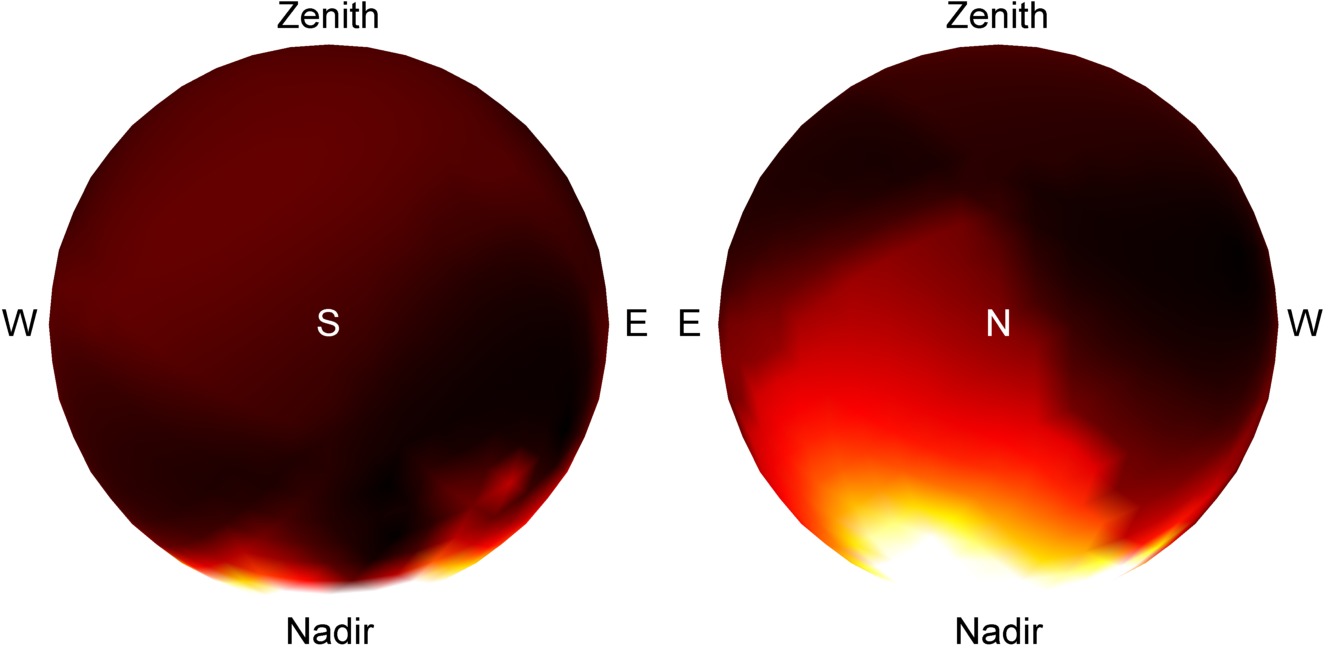
\includegraphics[width=.9\linewidth]{./figures/confidenceIntervals/20130824_10pm.png} \\
%     \vspace{-.8em} \noindent\rule{\linewidth}{0.1pt}
%     \begin{sideways}\begin{minipage}{.4\linewidth}\centering \scriptsize 11/06/2013 \\ 41\% sun visibility \vspace{5pt} \end{minipage}\end{sideways}
%     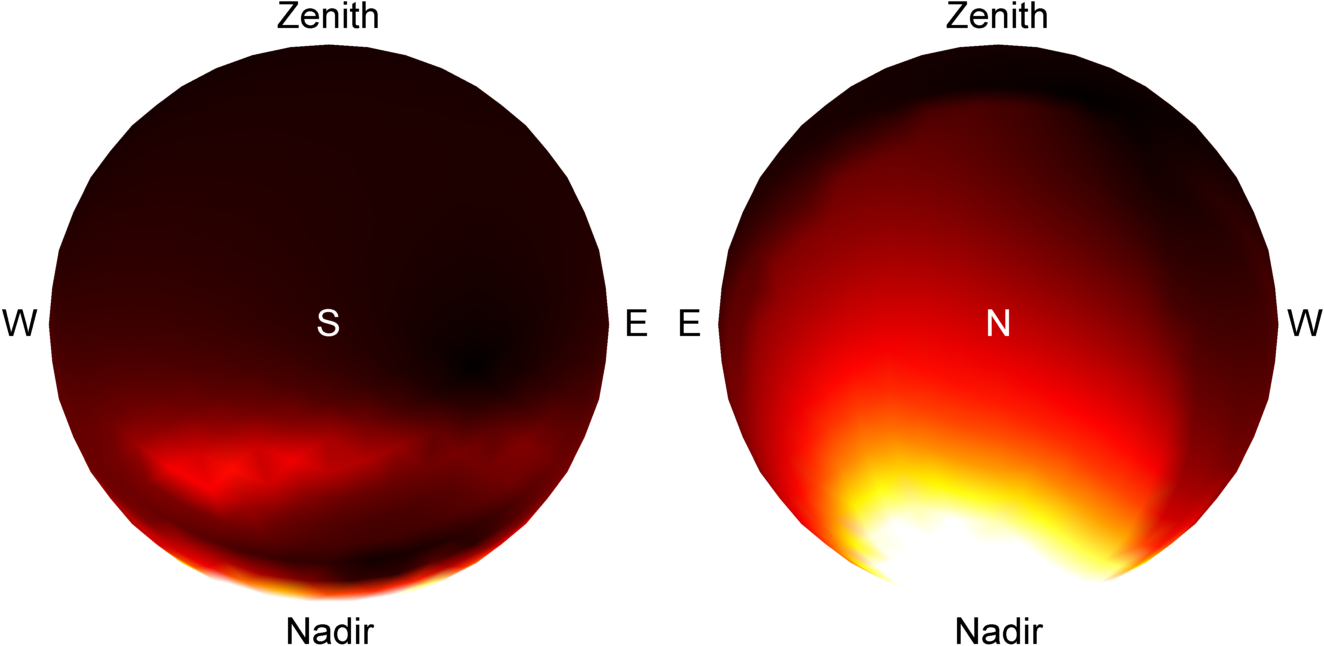
\includegraphics[width=.9\linewidth]{./figures/confidenceIntervals/20131106_10pm.png} \\
%     \vspace{-.8em} \noindent\rule{\linewidth}{0.1pt}
%     \begin{sideways}\begin{minipage}{.4\linewidth}\centering \scriptsize 11/08/2014 \\ 16\% sun visibility \vspace{5pt} \end{minipage}\end{sideways}
%     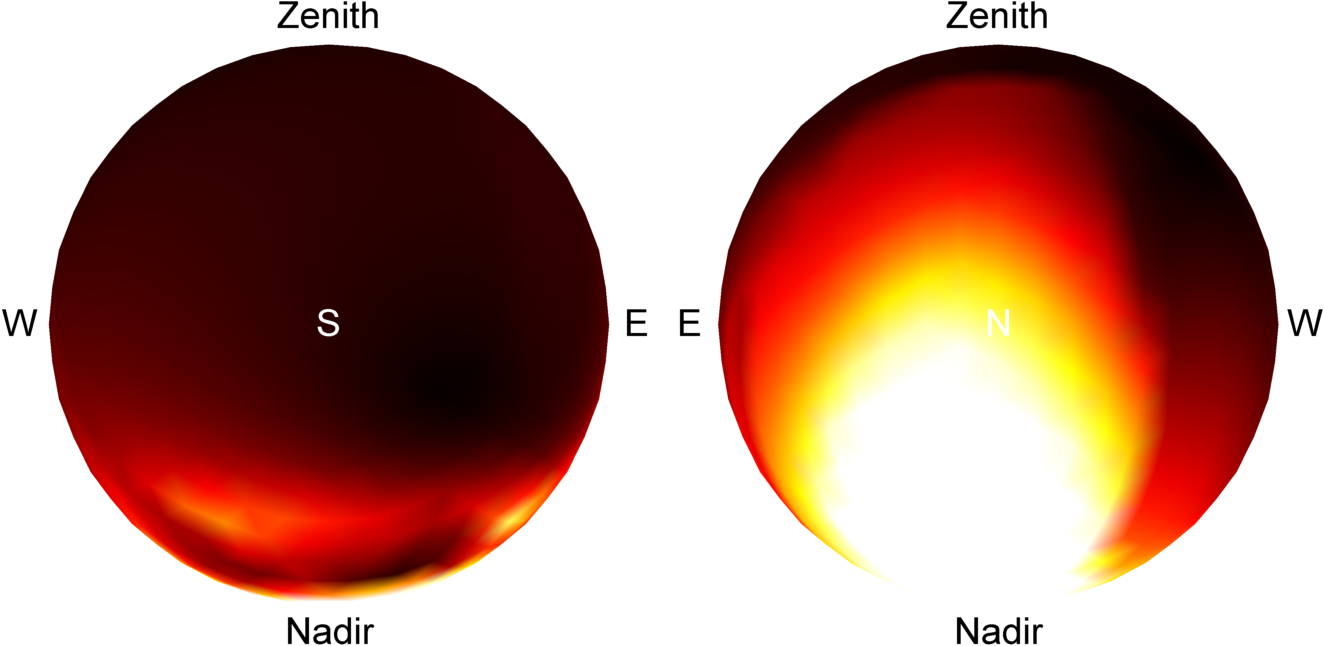
\includegraphics[width=.9\linewidth]{./figures/confidenceIntervals/20141108_10pm.png} \\
%     \end{minipage}
%     \vspace{3mm}
%     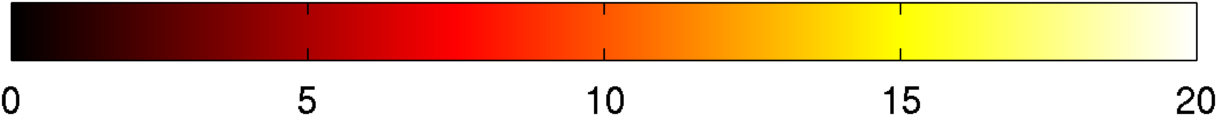
\includegraphics[width=.51\linewidth]{./figures/confidenceIntervals/colorbar.png}
%     \caption[Uncertainty in normal estimation in function of sun visibility]{Uncertainty in normal estimation with $\sigma=1\%$ is indicated by 95\% confidence intervals (in degrees), as a function of ground-truth surface normal. Results are shown for three different days in our dataset (same days as in fig.~\ref{fig:database}). The plots show the full sphere of normals from two different viewpoints: South (left), and North (right). Cardinal directions are shown for reference. The color-coding is indicated below the plots. See companion video for an animated version of these plots.}
%     \label{fig:confidence-intervals}
% \end{figure}

% \begin{figure*}[t]
%     \centering
%     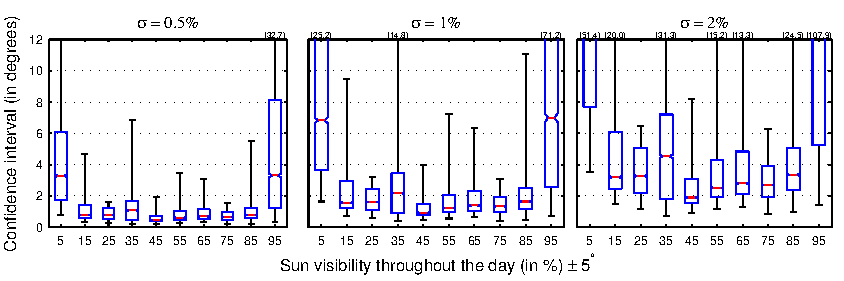
\includegraphics[width=.99\linewidth]{./figures/confidenceIntervals/sunVisibilityPlot-topHemisphere.pdf}
%     \vspace{-2mm}
%     \caption[Confidence interval of normal estimates in function of sun visibility]{Median confidence interval of normal estimates (red line) as a function of mean sun visibility over the course of the day for various values of $\sigma$. Our analysis predicts that normal reconstruction errors will likely be high if the sky is completely overcast (low sun visibility), or completely clear (high sun visibility). Good results can thus be expected in partially cloudy conditions, as shown in fig.~\ref{fig:cloud-cover}. The lower (upper) edge of each blue box indicates the 25th (75th) percentile. Statistics are computed only on normals pointing upwards to lessen ground effects.}
%     \label{fig:cloud-cover-plot}
% \end{figure*}


% \section{Computing the stability of outdoor PS}
% \label{iccp-computingstability}

% We aim to apply the stability analysis of sec.~\ref{sec:ch1_analysis} on all 23 days from our dataset, and on all possible normal directions. To do so, we consider each day independently, and first sample directions on the sphere by subdividing an icosahedron three times, yielding a set of 642 potential orientations $\mathcal{N} = \{\mathbf{n}_1, ..., \mathbf{n}_{642} \}$. Then, for each $\mathbf{n}_j \in \mathcal{N}$, we build the illumination matrix $\mathbf{L}$ in~\eqref{eqn:matrix-form}, given all 6 hours of data for that day. Finally, the 95\% confidence interval $\mathcal{C}_{\mathbf{n}_j}$ is computed using~\eqref{eqn:confidence-degrees}, indicating the uncertainty (possible reconstruction error) for that normal---the higher the interval, the less stable the solution.

% To compute $\mathcal{C}_{\mathbf{n}_j}$, values for the noise level $\sigma$ and the surface albedo $\rho$ from \eqref{eqn:confidence-xyz} must be chosen. For the albedo, we will consider the best case with $\rho=1$. To set $\sigma$, we first render noise-less pixel values $\mathbf{b}_j$ using the (ground-truth) normal ${\bf n}_j$ and~\eqref{eqn:matrix-form}, with ${\bf L}$ including our entire collection of environment maps. All figures have been generated with $\sigma$ set at $1\%$ of the 95th percentile value of the resulting $\mathbf{b}_j$, unless otherwise stated. This particular value is chosen to yield a small, yet non-negligible, level of noise that is similar to that in previous work~\cite{klaudiny-prl-14}. The values of $\rho$ and $\sigma$ are kept constant in order to focus solely on the influence of lighting conditions, but could be set to match particular experimental conditions if needed.

% Fig.~\ref{fig:confidence-intervals} shows the result of such an analysis on the three days of fig.~\ref{fig:database}. For each day, two sides of the sphere of normal directions are shown: seen from the South (left), and from the North (right). The spheres are color-coded according to the confidence interval $\mathcal{C}_\mathbf{n}$ for each normal direction. Note that vertex interpolation is used to display full spheres, but valid data is available only at vertices (thus the staircase effect in some plots).

% At first glance, we notice that normals pointing down (towards Nadir) consistently have high confidence intervals, irrespective of the illumination conditions. The stability of outdoor PS on these normals is thus expected to be low. This behavior concords with expectation: normals pointing down define integration domains $\Omega_{\mathbf{n}}$ (see fig.~\ref{fig:normal-diagram}) which mostly include the ground, whose intensity does not vary spatially throughout the day. Another interesting observation from fig.~\ref{fig:confidence-intervals} is that the same normal exhibits different confidence intervals depending on the day. This raises the question: what is the relation between outdoor illumination conditions and uncertainty in the recovered surface normal?


% \section{Influence of cloud cover}
% \label{sec:cloud-cover-results}

% It is already apparent from fig.~\ref{fig:confidence-intervals} that cloud coverage has an effect on the uncertainty of normal reconstruction, since an overcast day (last row) clearly does not behave the same way as a day with light clouds (top row). Here, we present a more systematic analysis of the influence of cloud coverage. To control for the effect of the sun elevation (which will be explored in sec.~\ref{sec:sun-elevation-results}), the analysis is performed on days with similar sun elevations by keeping only the skies captured in October and November.

% We approximate cloud coverage by computing the fraction of time that the sun is visible, \ie, that it fully shines on the scene, for a given day. To do so, we simply find the brightest spot in a sky image, and determine that the sun shines on the scene if the intensity of the brightest pixel is greater than $20\%$ of the maximum sun intensity---we determined empirically that this is the point at which the sun is bright enough to start creating cast shadows. Cloud coverage is represented by computing the mean sun visibility for a given day. A value of less than 10--15\% would indicate a mostly overcast sky, while skies are mostly clear with values above 85--90\%.

% \begin{figure}[t]
%     \centering
%     \begin{minipage}{.5\linewidth}
%     \begin{sideways}\begin{minipage}{.4\linewidth}\centering \scriptsize Clear (85-100\%)\vspace{5pt} \end{minipage}\end{sideways}
%     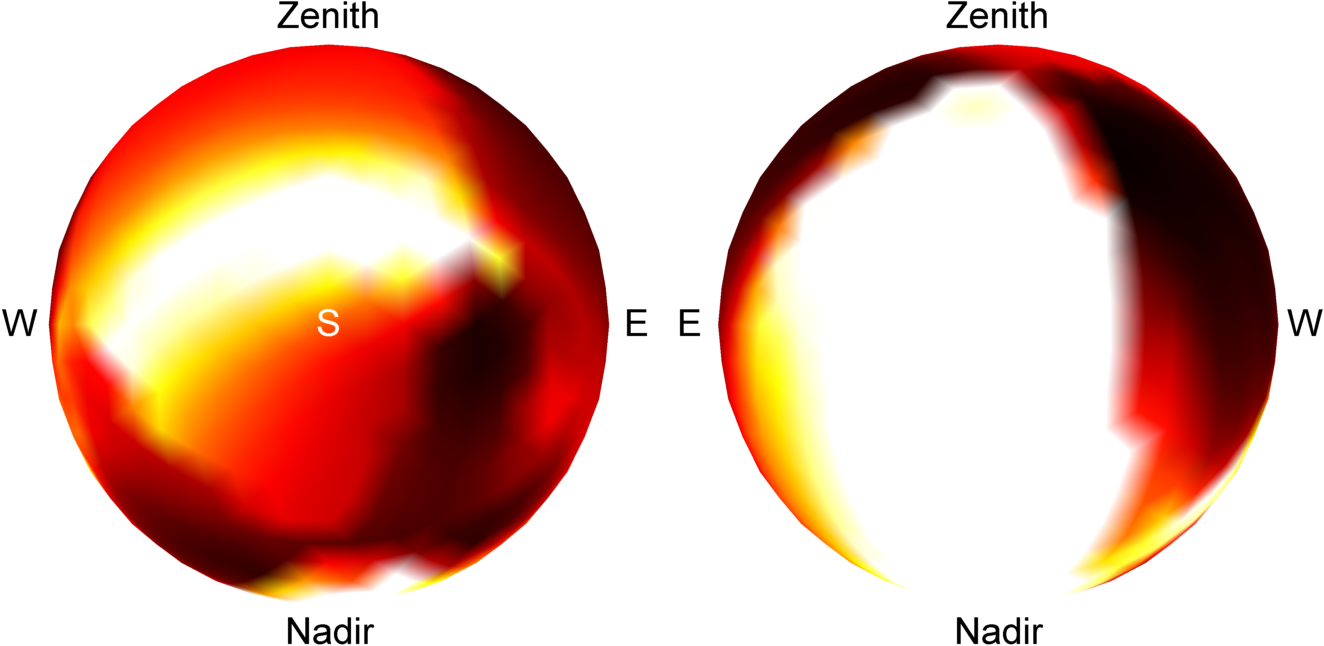
\includegraphics[width=.9\linewidth]{./figures/confidenceIntervals/clear-mean_10pm.png} \\
%     \vspace{.4em} \noindent\rule{\linewidth}{0.1pt} \vspace{-.8em}
%     \begin{sideways}\begin{minipage}{.4\linewidth}\centering \scriptsize Mixed Clear (50-85\%)\vspace{5pt} \end{minipage}\end{sideways}
%     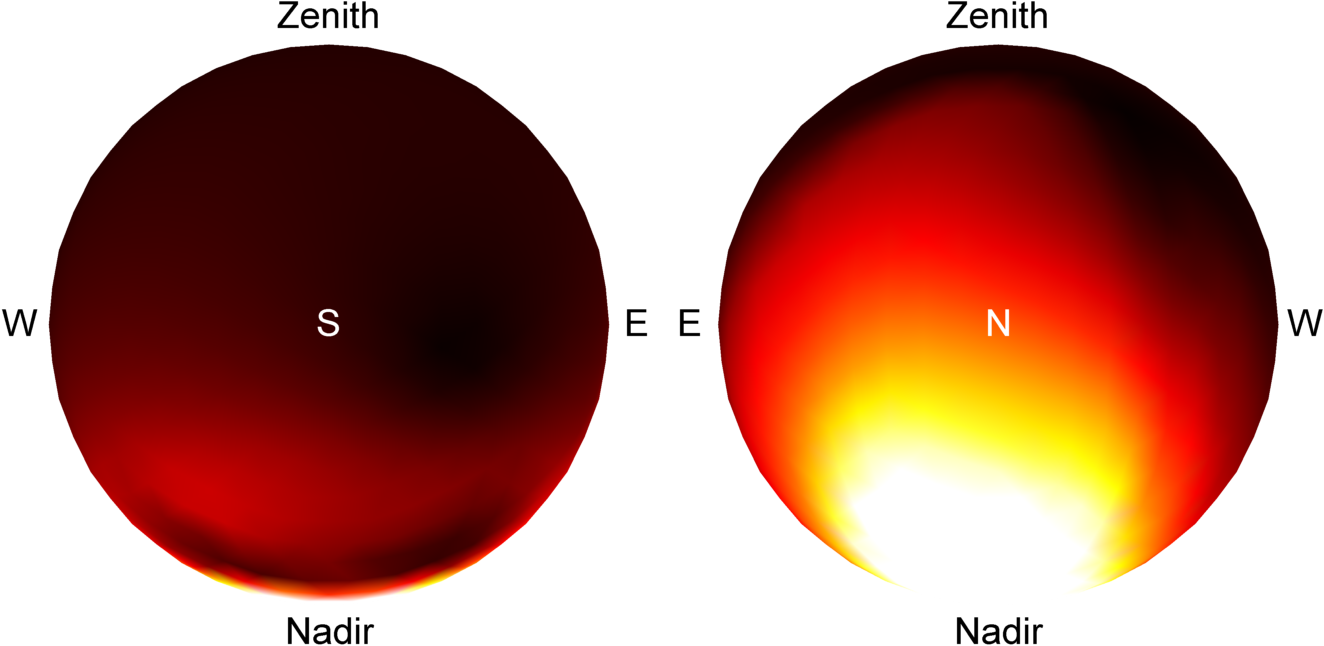
\includegraphics[width=.9\linewidth]{./figures/confidenceIntervals/mixed-clear-mean_10pm.png} \\
%     \vspace{.4em} \noindent\rule{\linewidth}{0.1pt} \vspace{-.8em}
%     \begin{sideways}\begin{minipage}{.4\linewidth}\centering \scriptsize Mixed Overcast (15-50\%)\vspace{5pt} \end{minipage}\end{sideways}
%     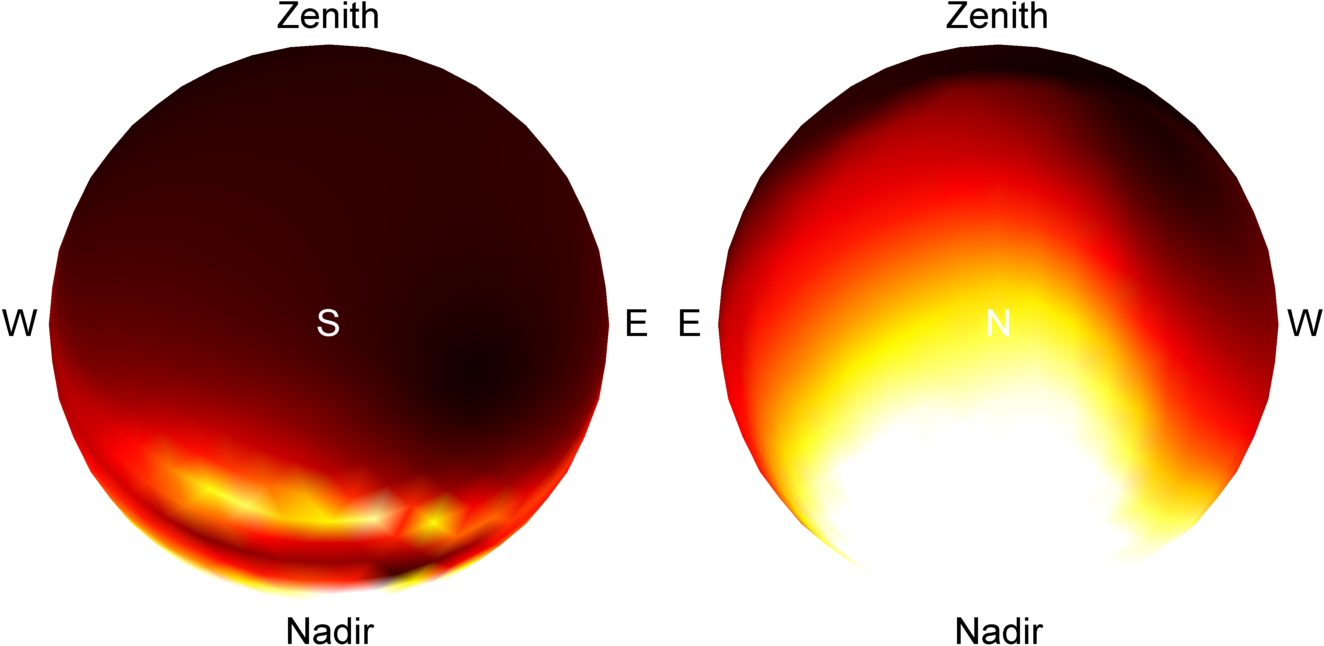
\includegraphics[width=.9\linewidth]{./figures/confidenceIntervals/mixed-overcast-mean_10pm.png} \\
%     \vspace{.4em} \noindent\rule{\linewidth}{0.1pt} \vspace{-.8em}
%     \begin{sideways}\begin{minipage}{.4\linewidth}\centering \scriptsize Overcast (0-15\%)\vspace{5pt} \end{minipage}\end{sideways}
%     \includegraphics[width=.9\linewidth]{./figures/confidenceIntervals/overcast-mean_10pm.png} \\
%     \end{minipage}
%     \vspace{3mm}
%     \includegraphics[width=.51\linewidth]{./figures/confidenceIntervals/colorbar.png}
%     \caption[Influence of cloud cover on confidence intervals]{Influence of cloud cover on the 95\% confidence intervals with $\sigma=1\%$. Each row shows a different type of sky, based on sun visibility. For example, the top row shows confidence intervals averaged over all days with direct sun visibility in the range 85\%-100\%. The averaged days presented similar sun elevations. As with fig.~\ref{fig:confidence-intervals}, the plots show the full sphere of normals from two different viewpoints: South (left), and North (right).}
%     \label{fig:cloud-cover}
% \end{figure}

% The relation between sun visibility and the confidence interval $\mathcal{C}_\mathbf{n}$ is shown in fig.~\ref{fig:cloud-cover-plot}. Normal reconstruction errors will likely be quite high in two situations: when the sky is completely overcast (low sun visibility), or completely clear (high sun visibility). Interestingly, good reconstruction results are expected for a wide range of cloud coverage conditions, ranging from 10--90\% mean sun visibility.

% These results are corroborated by fig.~\ref{fig:cloud-cover}, which shows the confidence intervals themselves on a plot similar to fig.~\ref{fig:confidence-intervals}. Results there are presented by averaging the intervals of skies belonging to four groups: overcast (0--15\%), mixed overcast (15--50\%), mixed clear (50--85\%), and clear (85--100\%) days. Again, high uncertainty results are visible for the two extreme cases of fully overcast and fully clear days, while the remainder indicate more stable solutions.

% % TODO: add figure to illustrate this (maybe)?
% The improved conditioning in mixed skies is explained by the following key observation: cloud cover shifts the mean light vectors ${\bf \bar l}_t$ towards zenith and away from sun trajectory in the sky. Therefore, even when the sun moves along a trajectory that nearly lies on a 3D plane, as shown in fig.~\ref{fig:mlv}, cloud cover effectively causes an {\em out-of-plane} shift of the mean light vectors, making reconstruction possible.

% \begin{figure}
%     \centering
%     \includegraphics[width=0.5\linewidth]{./figures/mlvFig/mlvFig.pdf}
%     \caption[Cloud effect on mean light direction]{Cloud effect on the mean light direction over one day: while the sun path (orange) yields nearly co-planar directions of illumination, the mean light directions (red dots) provide a much more varied set (data from 11/06/2013, 2nd row of fig.~\ref{fig:database}).}
%     \label{fig:mlv}
% \end{figure}

% This key observation also demonstrates the advantages of adopting more elaborate illumination models (\eg, \cite{yu-iccp-13}). For instance, the simpler point light model was used in \cite{shen-pg-14} to study the conditioning of outdoor PS. Because the atmospheric component is not modeled, the conclusion was that single-day reconstruction breaks down in two cases of nearly coplanar sun directions: closer to the poles near the winter solstice, and worldwide near an equinox. Our results suggest that more attention should be placed on the illumination model, without focusing exclusively on the sun.

% \section{Influence of sun elevation}
% \label{sec:sun-elevation-results}

% We also hypothesized the position of the sun to have an important effect on the ability to recover surface normals outdoors. Since our dataset is already aligned in terms of sun azimuths (see sec.~\ref{sec:hdrdb}), we now analyze the influence of sun elevation. For this purpose, we retain only the days for which the sun visibility was between 15--85\% of the time. We then compute the relation between sun elevation and expected reconstruction confidence, as illustrated in fig.~\ref{fig:sun-elevation-plot}.

% Sun elevation does appear to have an influence, with higher sun elevations resulting in slightly increased uncertainty than when the sun is lower in the sky. However, the impact is less drastic than that of cloud cover from sec.~\ref{sec:cloud-cover-results}. These results can be explained, at least in part, by the smaller sun-zenith shift introduced by cloud cover when the sun is already high in the sky; therefore, smaller improvements in conditioning are obtained.

% Our data-driven analysis shows that higher sun elevations---predicted as preferable by the analysis in~\cite{shen-pg-14}---are in fact not necessarily optimal when taking more elaborate illumination models into account.


% Section 3 has a note about non-coplanar sun directions  vs  non-coplanar mean light vectors (zenith, sun elevation),


% \section{Analyzing full objects}

% So far, our analysis has focused solely on one patch (one normal direction) at a time. But can we also say something about an entire object? Clearly, a full answer to this question would require analyzing non-local effects such as occlusions, inter-reflections, cast shadows, etc. However, we hypothesize that a simpler analysis ignoring these effects can still provide useful results. We therefore predict the performance of an outdoor PS algorithm by computing the expected value of the confidence interval, $\mathbb{E}_{\bf n}[\mathcal{C}_{\bf n}]$, over an entire object; expectation over the normal vector is computed using a prior distribution taken from a simpler convex shape (\eg, a sphere). Fig.~\ref{fig:objects} shows the expected reconstruction performance for two objects: a bottle, and the bunny. Overall, surface reconstruction performance is expected to be best when objects face south (\ie, the sun).

% \begin{figure}[t]
%     \centering
%     \includegraphics[width=\linewidth]{./figures/confidenceIntervals/sunElevationPlot-topHemisphere.pdf}
%     \caption[Confidence interval in function of sun elevation]{Median confidence interval of normal estimates (red line) as a function of maximum sun elevation over the course of the day for various values of $\sigma$. Although the effect is not as significant as with cloud cover, we anticipate a small decrease in performance at higher sun elevations. The lower (upper) edge of each blue box indicates the 25th (75th) percentile. Statistics are computed only on normals pointing upwards to lessen ground effects.}
%     \label{fig:sun-elevation-plot}
% \end{figure}

% \begin{figure}[t]
%     \centering
%     \begin{sideways}\begin{minipage}{.45\linewidth}\centering \scriptsize Low elevation \vspace{5pt} \end{minipage}\end{sideways}
%     \includegraphics[width=.9\linewidth]{./figures/confidenceIntervals/elevation-low-mean_10pm.png} \\[2mm]
%     \begin{sideways}\begin{minipage}{.45\linewidth}\centering \scriptsize High elevation \vspace{5pt} \end{minipage}\end{sideways}
%     \includegraphics[width=.9\linewidth]{./figures/confidenceIntervals/elevation-high-mean_10pm.png} \\[3mm]
%     \includegraphics[width=\linewidth]{./figures/confidenceIntervals/colorbar.png}
%   \caption{Influence of sun elevation on the 95\% confidence intervals with $\sigma=1\%$. The top plot shows the mean, per-normal, confidence intervals obtained for mixed skies with low sun elevation. The bottom plot shows the same data, but for mixed skies with high sun elevation. As in fig.~\ref{fig:confidence-intervals}, the plots show the full sphere of normals from two different viewpoints: South (left), and North (right). Cardinal directions are shown for reference. The color-coding is indicated below the plots.}
%   \label{fig:sun-elevation}
% \end{figure}

% \begin{figure}[t]
%     \centering
%     \includegraphics[width=\linewidth]{./figures/objectFig/objectFigNoise.pdf}
%     \caption[Example of object reconstruction performance]{Predicting object reconstruction performance for the 08/24/2013 dataset. These curves show the mean surface reconstruction variance for two objects: a bottle (blue) and the bunny (red). Irrespective of the noise level, surface reconstruction performance is expected to be best when the objects face south.}
%     \label{fig:objects}
% \end{figure}

% \subsection{Validation on real object images}
% \label{sec:validation}

% The analysis performed on our dataset indicates that surface patches may be better reconstructed in certain conditions, dependent upon cloud coverage, sun elevation, and the orientation of the patch itself. At the time of this writing, a thorough validation on real outdoor images of different objects is currently under development. This section reports preliminary results on real outdoor images of an owl statuette (fig.~\ref{fig:reconstruction:example_envmaps}), which was scanned with a Creaform MetraSCAN at a resolution of 0.05mm to provide a reference of true surface orientation.

% \begin{figure*}[!ht]
%     \centering
%     \setlength{\tabcolsep}{0pt}
%     \newcommand{\customwidth}{.077\linewidth}
%     \begin{tabular}{@{}rcccccccccccc@{}}
%     &
%     \begin{minipage}{\customwidth}\centering\scriptsize 10:30 \end{minipage} &
%     \begin{minipage}{\customwidth}\centering\scriptsize 11:00 \end{minipage} &
%     \begin{minipage}{\customwidth}\centering\scriptsize 11:30 \end{minipage} &
%     \begin{minipage}{\customwidth}\centering\scriptsize 12:00 \end{minipage} &
%     \begin{minipage}{\customwidth}\centering\scriptsize 12:30 \end{minipage} &
%     \begin{minipage}{\customwidth}\centering\scriptsize 13:00 \end{minipage} &
%     \begin{minipage}{\customwidth}\centering\scriptsize 13:30 \end{minipage} &
%     \begin{minipage}{\customwidth}\centering\scriptsize 14:00 \end{minipage} &
%     \begin{minipage}{\customwidth}\centering\scriptsize 14:30 \end{minipage} &
%     \begin{minipage}{\customwidth}\centering\scriptsize 15:00 \end{minipage} &
%     \begin{minipage}{\customwidth}\centering\scriptsize 15:30 \end{minipage} &
%     \begin{minipage}{\customwidth}\centering\scriptsize 16:00 \end{minipage}
%     \\
%     \begin{sideways}\begin{minipage}{\customwidth}\centering \scriptsize illumination \\ 43\% sun vis. \\ \vspace{5pt} \end{minipage}\end{sideways} &
%     \includegraphics[width=\customwidth]{./figures/reconstruction/envmaps/20141011_102928.jpg} &
%     \includegraphics[width=\customwidth]{./figures/reconstruction/envmaps/20141011_110128.jpg} &
%     \includegraphics[width=\customwidth]{./figures/reconstruction/envmaps/20141011_112928.jpg} &
%     \includegraphics[width=\customwidth]{./figures/reconstruction/envmaps/20141011_120128.jpg} &
%     \includegraphics[width=\customwidth]{./figures/reconstruction/envmaps/20141011_122929.jpg} &
%     \includegraphics[width=\customwidth]{./figures/reconstruction/envmaps/20141011_130128.jpg} &
%     \includegraphics[width=\customwidth]{./figures/reconstruction/envmaps/20141011_132928.jpg} &
%     \includegraphics[width=\customwidth]{./figures/reconstruction/envmaps/20141011_135928.jpg} &
%     \includegraphics[width=\customwidth]{./figures/reconstruction/envmaps/20141011_142928.jpg} &
%     \includegraphics[width=\customwidth]{./figures/reconstruction/envmaps/20141011_145928.jpg} &
%     \includegraphics[width=\customwidth]{./figures/reconstruction/envmaps/20141011_152928.jpg} &
%     \includegraphics[width=\customwidth]{./figures/reconstruction/envmaps/20141011_155928.jpg}
%     \\
%     \begin{sideways}\begin{minipage}{.106\linewidth}\centering \scriptsize object capture \\ \vspace{1em} \vspace{5pt} \end{minipage}\end{sideways} &
%     \includegraphics[width=\customwidth]{./figures/reconstruction/object/103307.jpg} &
%     \includegraphics[width=\customwidth]{./figures/reconstruction/object/110346.jpg} &
%     \includegraphics[width=\customwidth]{./figures/reconstruction/object/113346.jpg} &
%     \includegraphics[width=\customwidth]{./figures/reconstruction/object/120346.jpg} &
%     \includegraphics[width=\customwidth]{./figures/reconstruction/object/123346.jpg} &
%     \includegraphics[width=\customwidth]{./figures/reconstruction/object/130215.jpg} &
%     \includegraphics[width=\customwidth]{./figures/reconstruction/object/133215.jpg} &
%     \includegraphics[width=\customwidth]{./figures/reconstruction/object/135615.jpg} &
%     \includegraphics[width=\customwidth]{./figures/reconstruction/object/143215.jpg} &
%     \includegraphics[width=\customwidth]{./figures/reconstruction/object/150215.jpg} &
%     \includegraphics[width=\customwidth]{./figures/reconstruction/object/153215.jpg} &
%     \includegraphics[width=\customwidth]{./figures/reconstruction/object/160215.jpg}

%     \end{tabular}
%     \caption[Real data]{Real outdoor HDR images of owl statuette and corresponding HDR environment maps (top row) providing synchronized, high-fidelity estimates of illumination conditions. All images were acquired on 10/11/2014 and tone-mapped for display only (with $\gamma = 1.6$). The sun visibility was 43\% on this day. }
%     \label{fig:reconstruction:example_envmaps}
% \end{figure*}

% We oriented this owl statuette towards south and took 66 HDR captures using a Canon EOS Rebel SL1 between 10h30 and 16h30, local time, in Quebec City. These captures were synchronized with the HDR environment maps described in sec.~\ref{sec:hdrdb}, providing high fidelity estimates of the illumination conditions for each image, as shown in fig.~\ref{fig:reconstruction:example_envmaps}. The laser scan was then manually aligned to these images.

% A simple outdoor PS algorithm was run on evenly distributed patches on the owl images. For each patch, the surface normal is obtained as to minimize the rendering error given by the model in~\eqref{eqn:matrix-form}, in a least-squares sense. Since this estimation problem is nonlinear on the normal ${\bf n}$, a solution is computed via exhaustive search on a set of 271 candidate orientations for the light hemisphere $\Omega_{\bf n}$. Given $\Omega_{\bf n}$, a candidate solution ${\bf x}$ is obtained via linear least squares. For the best solution, an estimation error, in degrees, is computed using the reference normal from the laser scan. The uncertainty measure (confidence interval $\mathcal{C}_{\bf n}$) derived in sec.~\ref{subsec:measure_uncertainty} is also computed for each patch.

% Results from this quantitative evaluation are given in fig.~\ref{fig:reconstruction:results}. As shown on the left, normals pointing upwards are generally recovered more accurately than normals pointing downwards. This is in concordance with the predicted confidence intervals shown on the right in fig.~\ref{fig:reconstruction:results}. The behavior of the reconstruction error is, in general, well predicted by the confidence intervals.
% % Note however that the ground truth normals were aligned with the images manually, therefore slight misalignments could explain discrepancies.


% \begin{figure}[t]
%     \centering
%     \begin{minipage}{0.5\linewidth}
%     \newcommand{\customwidthres}{0.45\linewidth}
%     \begin{tabular}{cc}
%         \scriptsize Angular differences to ground truth & \scriptsize Predicted 95\% confidence intervals \\
%         \includegraphics[width=\customwidthres]{./figures/reconstruction/owl_delta_gt.png} &
%         \includegraphics[width=\customwidthres]{./figures/reconstruction/owl_confint.png}
%         \begin{picture}(0,0)
%             \put(-155,-2){\includegraphics[height=1.5cm]{./figures/reconstruction/owl_sphere_dgt.png}}
%             \put(-35,-2){\includegraphics[height=1.5cm]{./figures/reconstruction/owl_sphere_ci.png}}
%         \end{picture}
%     \end{tabular}
%     \includegraphics[width=1.01\linewidth]{./figures/reconstruction/colorbar.png}
%     \end{minipage}
%     \caption[Qualitative validation on images of a real object]{Quantitative validation on images of a real object. Evenly distributed patches of the owl images were used to perform a simple calibrated outdoor PS algorithm. Error estimates of the surface normals are reported on the left using the reference surface orientation in the laser scan. The predicted 95\% confidence intervals $\mathcal{C}_\mathbf{n}$ from \eqref{eqn:confidence-degrees} are shown on the right. A few large estimation errors on the left image may be caused by imperfect alignment between the scanned model and the images. Insets in the lower right corner show the recovered normals mapped to the south hemisphere. Normals in dark blue means no data available.}
%     \label{fig:reconstruction:results}
% \end{figure}


% !TEX root = main.tex


%\subsection{Outdoor PS conditioning}
%\label{sec:sensitivity-analysis}

%In the following, we consider a small planar surface patch with normal vector ${\bf n}$ and Lambertian reflectance with albedo~$\rho$. As discussed in~\cite{holdgeoffroy-iccp-15,hung-wacv-15}, the lighting contribution of an environment map to a Lambertian surface patch can be formulated as in an equivalent problem with a single point light source $\bar{\mathbf{l}} \in \mathbb{R}^3$. This vector is the mean of the light vectors computed over the hemisphere of incoming light directions defined by ${\bf n}$. This virtual point light source $\bar{\mathbf{l}}$ is henceforth referred to as the {\em mean light vector} (MLV). It is important to note that, as opposed to the traditional PS scenario where point light sources are fixed and thus independent of ${\bf n}$, here the {\em per-pixel} MLV is a function of $\mathbf{n}$. Thus, patches with different orientations define different sets of MLVs (as discussed later and shown in fig.~\ref{fig:realShiftNormal}).

%the lighting contribution of an environment map to a Lambertian surface patch can be formulated as in an equivalent problem with a single point light source $\bar{\mathbf{l}} \in \mathbb{R}^3$. This vector is the mean of the light vectors computed over the hemisphere of incoming light directions defined by ${\bf n}$. This virtual point light source $\bar{\mathbf{l}}$ is henceforth referred to as the {\em mean light vector} (MLV). It is important to note that, as opposed to the traditional PS scenario where point light sources are fixed and thus independent of ${\bf n}$, here the {\em per-pixel} MLV is a function of $\mathbf{n}$. Thus, patches with different orientations define different sets of MLVs (as discussed later and shown in fig.~\ref{fig:realShiftNormal}).

%Given multiple images of the same patch, taken at different times, we collect all photometric constraints for that patch and obtain the PS equation in matrix form:
%
%\begin{equation}
%\mathbf{b} =
%\begin{bmatrix}
% b_1 \\ b_2 \\ \vdots \\ b_T
%\end{bmatrix}
%= 
%\begin{bmatrix}
% {\bf \bar l}_1^T \\ {\bf \bar l}_2^T \\ \vdots \\ {\bf \bar l}_T^T
%\end{bmatrix}
%{\bf x} = \mathbf{L} \mathbf{x} \,,
%\label{eqn:matrix-form}
%\end{equation}
%
%where $b_i \in \mathbb{R}$ are the observed pixel intensities, and ${\bf x} \in \mathbb{R}^3$ is the surface normal ${\bf n}$ scaled by $\rho$.

%Let $\hat{{\bf x}}=({\bf L}^T{\bf L})^{-1}{\bf L}^T{\bf b}$ denote the least-squares solution of~\eqref{eqn:matrix-form}. A 95\% confidence interval for normal ${\bf x}$ is given by 
%
%\begin{equation}
%\hat{\mathbf{x}} \pm \bolddelta \,, \quad \text{with } \delta_k = 1.96 \frac{\sigma}{\rho}\lambda_k \,,
%\label{eqn:confidence-xyz}
%\end{equation}
%
%where $\sigma$ is the camera noise level and $\lambda_k$ is the square root of the $k$-th element on the diagonal of $({\bf L}^T{\bf L})^{-1}$~\cite{hastie-book-09}. 

% A more intuitive measure of uncertainty in the estimate $\hat{{\bf n}}$ is obtained by considering angular distances $\theta$ in degrees, 
% % 
% \begin{equation}
% \theta^\pm = \cos^{-1}({\bf \hat n}^T{\bf \hat n}^\pm)\,, 
% \quad \text{where }
% {\bf \hat n}^\pm = \frac{{\bf \hat n} \pm \bolddelta}{\lVert{\bf \hat n} \pm \bolddelta \rVert}.
% \label{eqn:angular-dist}
% \end{equation}
% %
% Our measure of uncertainty, or stability, in the estimation of ${\bf \hat n}$ is then defined as the confidence interval \mbox{$\mathcal{C}_{\bf n} = [ 0, \max(\theta^\pm) ]$} in degrees.

% In the analysis below, we often take the estimate ${\bf \hat n}$ to be the ground truth normal ${\bf n}$ of a simulated (synthetic) surface patch; this corresponds to the result of an ideal algorithm. We then evaluate the confidence interval for this normal using a set of real, outdoor environment maps with associated stability parameters $\lambda_k$ as in~\eqref{eqn:confidence-xyz}. The result is a measure of the uncertainty in the reconstruction that an actual outdoor PS algorithm would provide on that particular set of illumination conditions, and surface orientation. As in~\cite{holdgeoffroy-iccp-15}, our simulations below consider synthetic surface patches with albedo $\rho = 1$ and a small, non-negligible noise level $\sigma$ at $1\%$ of the maximum pixel value.


%\section{Analysis of $x$-hour outdoor PS}
\section{Theoretical analysis of mean light vectors}
\label{sec:ch1_analysis}

In this section, we seek what is the minimum capture interval required by PS to work. We do so by tying what is happening in the sky to reconstruction performance. The analysis is done on images that were captured during a continuous 6 hour time interval on each of these days, from 10:30 until 16:30.\footnote{Companion video showing data samples available at \url{http://vision.gel.ulaval.ca/~jflalonde/projects/xHourPS/} and \url{http://vision.gel.ulaval.ca/~jflalonde/projects/outdoorPS/}.} 

From the 95\% confidence interval defined in eq.~\eqref{eqn:confidence-xyz}, we can deduce that the only light-dependent stability factor in the confidence interval $\bolddelta$ is $\lambda_k$; the other two factors are related to the camera ($\sigma$), and surface reflectance~($\rho$). In the remaining of this chapter, we analyze the maximum uncertainty \mbox{$\lambda_\text{max} = \max_k(\lambda_k)$}, as a conservative performance measure that is independent of albedo and sensor noise; $\lambda_\text{max}$ is a {\em maximum noise gain} factor, \ie, the intensity of noise amplification in the solution. Here, we are interested in 1) investigating how the noise gain $\lambda_\text{max}$ is influenced by the duration of outdoor data capture, and in 2) identifying specific changes, or {\em events}, in outdoor lighting that are associated with more stable PS solutions (smaller $\lambda_\text{max}$).

To make our analysis tractable, we do not model cast shadows and inter-reflections. In addition, we assume that the sky hemisphere (around zenith) provides the dominant part of incoming light. Unless stated otherwise, our simulations consider a day near an equinox, which corresponds to the worst case scenario with coplanar sun directions~\cite{shen-pg-14}.

This section provides the first answers to the questions raised above by looking at collections of mean light vectors (MLVs) as defined in~\ref{iccp15:ifm} from both simulated and real sky data. The main goal is to analyze the behavior of the illumination factors $\lambda_k$ (and associated confidence interval) of normal estimation. More specifically, we investigate numerical stability (MLV coplanarity) as a function of the apparent sun motion and cloud coverage within capture intervals of different durations, containing different atmospheric events. We also compare the resulting performance measures of $x$-hour outdoor PS to those of full-day outdoor PS.

% Here our goal is to answer the questions: \emph{what} are the important changes, or {\em events}, in outdoor lighting that affect $\lambda_k$? What is the minimum duration of data capture, containing one or more of such events, that can lead to performance similar to that of full-day PS?

% -----------------------------------------------------------------------------
\begin{figure}[t]
\centering
\includegraphics[width=.33\columnwidth]{diagram_MLVshift3}
\caption[Impact of cloud coverage on PS conditioning]{Impact of cloud coverage on the numerical conditioning of outdoor PS: clear (a) and overcast (b) days present MLVs with stronger coplanarity; in partly cloudy days (c) the sun is often obscured by clouds, which may lead to out-of-plane shifts of MLVs.}
\label{fig:MLVshift}
\end{figure}
% -----------------------------------------------------------------------------
% -----------------------------------------------------------------------------
\begin{figure*}[t]
\centering
\includegraphics[width=.32\textwidth]{v123gainSurf} \ \ \ %\\[3mm]
\includegraphics[width=.32\textwidth]{v123gain1Arc} \ \ \ %\\[3mm]
\includegraphics[width=.32\textwidth]{v123gain2Shift}
\caption[Simulated noise gain as function of solar arc and mean light vector shift]{Simulated noise gain $\lambda_{\max}(\theta_a,\theta_e)$ as a function of solar arc $\theta_a$ and MLV shift (elevation) angle $\theta_e$. See discussion in the text.}
\label{fig:v123gain}
\end{figure*}
% -----------------------------------------------------------------------------

\subsection{Cloud coverage and MLV shifting}
\label{subsec:mlv-clouds}

Under clear skies, the MLVs of the model above will point nearly towards the sun, from which arrives most of the incoming light. Thus, near an equinox (worldwide), the resulting set of MLVs are nearly coplanar~\cite{shen-pg-14}, resulting in poor performance, fig.~\ref{fig:MLVshift}(a). For a day with an overcast sky, performance is also poor because the set of MLVs are nearly colinear and shifted towards the patch normal ${\bf n}$, fig.~\ref{fig:MLVshift}(b). Finally, in partly cloudy days (mixed skies), the sun is often obscured by clouds and such occlusion shifts some MLVs away from the solar plane, improving numerical stability, fig.~\ref{fig:MLVshift}(c). 

% NOT SURE ABOUT THIS ANYMORE:
% This improvement in conditioning is more significant with lower sun elevations, as the MLVs are shifted towards zenith.


\subsection{Solar arcs and MLV elevation}
\label{subsec:solararcs-mlvelevation}

%If we assume equinox, then the sun actually moves on a plane worldwide (i.e. independent of latitude) and is also visible 12 hours worldwide (although terrain and atmosphere play a small role and change that). Thus, this simulation requires the equinox assumption. What does vary with latitude (at equinox) is: (1) the inclination of the solar plane, and (2) the frequency of cloud coverage (if the sun is lower in the sky most of the day). Anything else?

Here, we seek to provide a sense of the minimal length of solar arc and amount of out-of-plane MLV shift required in single-day outdoor PS. 

Assuming a day near an equinox, the apparent sun trajectory worldwide describes an arc $\theta_a$ within the solar plane of about $15^\circ$ per hour. We now use this observation to evaluate the numerical stability of outdoor PS for data capture intervals (solar arcs) of different lengths. Considering a partly cloudy sky, we also investigate the interaction of solar arc and cloud coverage; we quantify performance as a function of both acquisition time (solar arc $\theta_a$) and amount of out-of-plane MLV shift (elevation angle $\theta_e$) introduced by clouds.

A simple and effective way to investigate conditioning with different capture scenarios is to consider a simulation with the minimum number of three MLVs, as required for outdoor PS using~\eqref{eqn:matrix-form}. We simulate solar arcs $\theta_a$ of different lengths by defining two MLVs on a reference solar plane, with the third MLV presenting varying elevation $\theta_e$ away from this plane, as illustrated in fig.~\ref{fig:MLVshift}(c). The actual orientation of the solar plane varies with the latitude of the observer; thus, we represent MLV shift relative to this plane.

The numerical conditioning of outdoor PS, as observed with different configurations for these three MLVs, is then scored using the noise gain~$\lambda_{\max}$ (sec.~\ref{sec:modeling_uncertainty}). This measure is independent of albedo and sensor noise; it is also related to the condition number of the illumination matrix ${\bf L}$ in~\eqref{eqn:matrix-form}.

% Lower bound as MLV intensity is reduced by cloud coverage; thus MLV elevation need to be higher, actually.

% define full day as 6-hour outdoor PS (shadowing concerns)?

We compute~$\lambda_{\max}(\theta_a,\theta_e)$ for solar arcs $\theta_a$ of up to 6 hours ($90^\circ$) and MLV elevations $\theta_e$ up to $90^\circ$. For simplicity, we consider triplets of unit-length MLVs---thus, conditioning depends on the magnitude $\sin(\theta_e)$ of the out-of-plane component of the third MLV. Clearly, the optimal noise gain~$\lambda_{\max} = 1$ is obtained when the MLVs are mutually orthogonal ($\theta_a = \theta_e = 90^\circ$).

Fig.~\ref{fig:v123gain}(a) shows that the noise gain $\lambda_{\max}$ drops quickly to under 6 for capture intervals at just above 1 hour and for MLV shifts $\theta_e > 15^0$. This result suggests that even the performance of 1-hour PS can be acceptable with small levels of sensor noise $\sigma$ and high surface reflectance $\rho$. To ease visualization, figs.~\ref{fig:v123gain}(b,c) show cross sections of the $\lambda_{\max}(\theta_a,\theta_e)$ gain surface for a constant shift or solar arc.

A second important prediction from fig.~\ref{fig:v123gain}, considering (more realistic) small to moderate amounts of MLV shifts $\theta_e \leq 40^\circ$, is that conditioning will improve very little for data capture intervals above 3 hours ($45^\circ$ solar arcs). Reducing data capture from 3 to 2 hours would lead to an additional increase in uncertainty ($\lambda_{\max}$) of less than $30\%$ (from about 2.8 to nearly 3.6). Still, 2-hour outdoor PS with noise gains under $4\times$ may be possible if an MLV shift of $\theta_e > 20^\circ$ is introduced by atmospheric events during capture. Uncertainty in the results of 1-hour outdoor PS would be about 5 to 7 times that of full-day (6-hour) outdoor PS.


\section{Mean light vector shifts in real sky probes}

% how much MLV shift is expected?
% but how much uncertainty can we expect? look into real sky probes...
% Here we evaluate the actual noise gain from real data... 
% pick days near equinox to isolate shifting due to clouds only (really needed?)
% TODO: What happens with natural sun elevation in summer (non-equinox), high-latitude? sun declination angle of $23.5^\circ$. The other two vectors are always on plane!

% what we do: look at gain to infer elevation, we fit solar arc for clear sky, look at orthogonal component of MLVs
% for each normal visible to the camera, we plot the best gain computed from the solar plane and a third MLV
% does enough shift really happen? how much shift and for which normals?
% average/pattern over multiple days?

While the analysis above suggests that outdoor PS may be possible with a capture interval of only about 1 to 3 hours, it does not answer whether it is possible to observe an adequate amount of MLV shift (elevation away from solar plane) within a single partly cloudy day. In the following, we analyze the shifting (coplanarity) of real MLVs obtained from the database of real environment maps (sky probes) presented in sec.~\ref{sec:hdrdb}.

% MLV shifting depends on which portion of the sky the normal (patch) sees.
% shifting varies with normal (examples, more in suppl video)
% dimming in overcast (early morning/afternoon) affects conditioning too (explain)

First, it is important to note that surface patches of different orientations (normals) are exposed to different hemispheres of illumination, with light arriving from above (sky) and below (ground). This fact is illustrated in fig.~\ref{fig:realShiftNormal} for three different normal vectors (rows) and two different days (columns). Each globe represents the coordinate system for the environment maps captured in a day. For each combination normal-day, the time-trajectory of computed MLV directions (dots) and intensities (colors) are shown on the globe. Brighter MLVs lie closely to the solar arc, while darker MLVs may shift away from it. Note that we present normals that are mainly southward as they receives the most direct sunlight throughout the day in the Northern hemisphere. Surfaces with normals pointing north, for example, would be in shadow throughout the day in latitudes higher than the Tropic of Cancer around the winter solstice. As such, for the remainder of this chapter, we consider a camera that points toward north.

To more closely match the scenario considered above, we scale these real MLVs so that the brightest one over all days (\ie, for the most clear sky) has unit-length. From fig.~\ref{fig:realShiftNormal}, also note that some MLVs are shifted very far from the solar arc but, as indicated by the darker colors, their intensity is dimmed considerably by cloud coverage; little improvement in conditioning is obtained from these MLVs. 

Most important, fig.~\ref{fig:realShiftNormal} shows that the amount of out-of-plane MLV shift (elevation) relative to the solar arc also depends on the orientation ${\bf n}$ of the surface patch. This suggest that outdoor PS reconstruction may present different amounts of uncertainty (conditioning) depending on the normal of each patch. Indeed, the noise gain ($\lambda_{\max}$) values in fig.~\ref{fig:realShiftAll} show that patches with nearly horizontal normals (orthogonal to the zenith direction) are associated with sets of MLVs that are closer to being coplanar throughout the day. As expected, patches oriented towards the bottom also present worse conditioning since they receive less light. 

% Normals nearly horizontal are worse, why? Interesting!
% Uncertainty is higher, more errors, suggest direction for future investigation

Although these MLVs were computed from environment maps captured in the Northern hemisphere (Pittsburgh, USA, and Quebec City, Canada~\cite{holdgeoffroy-iccp-15}), similar conclusions can be drawn for the Southern hemisphere. Finally, note that this section has considered MLV shifts in whole-day datasets. Next, we look at subsets of MLVs from time intervals of varying lengths and analyze some of the atmospheric events associated with improved conditioning. 

% Next, we look into real datasets of partly cloudy skies and measure the actual amount of MLV shifting for hypothetical capture sessions of varying duration, from 1 to 6 hours. 


% -----------------------------------------------------------------------------
\begin{figure}[t]
\centering
\hspace{3.1cm} \includegraphics[width=2.6cm]{sphere_key_bold} \\[-1mm]
\includegraphics[height=1.43in]{sphereShift20131106_n1} \ \ %\\[3mm]
\includegraphics[height=1.43in]{sphereShift20141011_n1} \\[3mm]
\includegraphics[height=1.43in]{sphereShift20131106_n2} \ \ %\\[3mm]
\includegraphics[height=1.43in]{sphereShift20141011_n2} \\[3mm]
\includegraphics[height=1.43in]{sphereShift20131106_n3} \ \ %\\[3mm]
\includegraphics[height=1.43in]{sphereShift20141011_n3} \\[2mm]
{\footnotesize {\verb| |} \hspace{0.5cm} (a) Mixed clouds (06-NOV-13) \hspace{0.25cm} (b) Mixed clouds (11-OCT-14) }\\
%\vspace{-2mm}
\caption[Examples of mean light vectors in function of the normal studied]{Globes representing the coordinate system of sky probes. Each normal (blue arrow) defines a shaded hemisphere in the environmental map that does not contribute light to the computed MLVs (dots). All MLVs in two particular partly cloudy days (columns) were computed from real environment maps~\cite{holdgeoffroy-iccp-15} for 3 example normal vectors (rows). Relative MLV intensities are shown in the color bar on the left. See also video in~\cite{webpageXhourPS}.}
\label{fig:realShiftNormal}
\end{figure}
% -----------------------------------------------------------------------------
% -----------------------------------------------------------------------------
\begin{figure}[!ht]
\centering
\includegraphics[height=1.46in]{sphereGain20131106} \ \ \ %\\[3mm]
\includegraphics[height=1.46in]{sphereGain20141011} \\[1mm]
{\footnotesize {\verb| |} \hspace{.6cm} (a) 06-NOV-13 \hspace{1cm} (b) 11-OCT-14 }\\[3mm]
%\vspace{-2mm}
\caption[Noise gain over the sphere]{Noise gain for each normal direction ${\bf n}$ visible to the camera; the colors indicate the shifting (coplanarity) of the associated MLVs. The camera is assumed to lie to the South of this hypothetical target object. For both days, normals that are nearly horizontal are associated with more coplanar MLVs (smaller shifts, higher gains). These normals define a {\em zero-crossing region} between positive and negative out-of-plane shifts (mid row in fig.~\ref{fig:realShiftNormal}), where occlusion of the sun results in shifts that are predominantly {\em along} the solar arc. See also video available in~\cite{webpageXhourPS}.}
\label{fig:realShiftAll}
\end{figure}
% -----------------------------------------------------------------------------


\subsection{Analyzing time intervals}

In this section, we show how the conditioning of outdoor PS evolves over time. Analyzing the patterns in its evolution will allow us to isolate important ``events''---points at which uncertainty suddenly drops---and investigate whether such events occur in close succession.

The main results are given in fig.~\ref{fig:events}, which plots the gain factor $\lambda_{\max}$ for all possible time intervals in four different days. Since $\lambda_{\max}$ varies with ${\bf n}$, we plot the median gain over 321 normal vectors visible to the camera (by subdividing an icosahedron three times) for each time interval.

The first row of fig.~\ref{fig:events}(a,b) illustrates the case of two days identified in sec.~\ref{subsec:mlv-clouds} as yielding poor outdoor PS reconstructions. As seen in the plots, low noise gains are never reached, irrespective of the start time and duration of the capture interval. We note that the (nearly) overcast sky of fig.~\ref{fig:events}(b) exhibits better behavior than the completely clear sky of fig.~\ref{fig:events}(a). This is because that day is not completely overcast, and the sun sometimes becomes visible (see the sun log-intensity plot). MLVs are thus shifted away from their main axes, while improving conditioning only slightly.

More interesting scenarios arise on days exhibiting a better mix of sun and moving clouds, such as the two examples in fig.~\ref{fig:events}(c,d). The two black vertical lines in fig.~\ref{fig:events}(c) identify capture intervals starting at two different times. Following the line labeled ``start time 1'' (beginning at 11:00), we notice that uncertainty remains high for approximately two hours, then suddenly drops at around 13:00. This time instant is followed by sudden changes in sun intensity (due to passing clouds) that are sufficient to shift the MLV away from the sun plane. Subsequently, uncertainty continues to decrease, albeit at a much slower pace, over the rest of the day. The second time interval (identified as ``start time 2'') starts at 14:00, so it does not benefit from that period of sun intensity changes. The maximum gain at the end of the interval is therefore higher. 

Of course, this could be due to a simple fact: the first interval is longer than the second one. However, fig.~\ref{fig:events}(d) shows that longer intervals do not always result in lower uncertainty. This time, two 2-hour intervals are considered. The time interval labeled as ``start time 1'' stops right before the 14:00 mark, and only sees clear skies; as expected, the uncertainty is very high. ``Start time 2'', beginning at 13:30, can fully exploit the MLV shifts caused by moving clouds to dramatically decrease PS uncertainty, even while the interval length is kept constant.
  
\begin{figure*}[!th]
\centering
\footnotesize
\setlength{\tabcolsep}{0pt}
\begin{tabular}{cc}
\includegraphics[height=4.7cm]{./figures/events/events-20141003-colorbar.pdf} & 
\includegraphics[height=4.7cm]{./figures/events/events-20131119-colorbar.pdf} \\
(a) Clear day (03-OCT-14) & (b) Nearly overcast day (19-NOV-13) \\%*[.5em]
% \multicolumn{2}{c}{\includegraphics[width=.3\linewidth]{./figures/events/colorbar-horizontal-withlegend.pdf}} \\%*[.5em]
\includegraphics[height=4.7cm]{./figures/events/events-20130824-colorbar.pdf} & 
\includegraphics[height=4.7cm]{./figures/events/events-20131106-colorbar.pdf} \\
(c) Clear sky and mixed clouds (24-AUG-13) & (d) Mixed clouds (06-NOV-13)
\end{tabular}
\vspace{.25em}
\caption[Fine-grained analysis of PS uncertainty]{Fine-grained analysis of the expected uncertainty of outdoor PS as a function of time over four selected days in the dataset. Colored plots show the maximum gain $\lambda_\text{max}$ as a function of start time (diagonal along the plot), and duration of the interval. The black lines identify particular time intervals discussed in the text. The blue curve to the left of each colored plot represents the log sun intensity over the course of that day. Photographs of the sky for each day are also shown on the left.}
\label{fig:events}
\end{figure*}

\subsection{Overall performance of $x$-hour PS} 

We noted in fig.~\ref{fig:events}(d) that sufficient conditions for low uncertainty could be met in as little as 2 hours. In this section, we evaluate how often one can achieve low uncertainty in short time intervals. This is done by assessing the distribution of noise gains from short time intervals, and aggregating results over multiple days.

To compute these statistics, we first consider a single normal and a single day. For a particular time interval \mbox{$\tau = \{t_\text{start}, t_\text{end}\}$}, we compute the ratio $r_\lambda(\tau)$ of its noise gain divided by the best (minimum) gain of all possible intervals in this day (including the full-day interval). Fig.~\ref{fig:ratios}(a,b) shows distributions of relative gains $r_\lambda$ for the two days in fig.~\ref{fig:events}(c,d). Fig.~\ref{fig:ratios}(a) shows that, for intervals of 4 hours, 75\% of the normals have uncertainty below twice the minimum gain for that day. In the case of fig.~\ref{fig:ratios}(b), that interval drops to 3 hours. 

The ratios $r_\lambda$ were then computed for all normals, over all days in the database. The compound statistics are shown in fig.~\ref{fig:ratios}(c). They empirically illustrate that there were many opportunities for stable normal reconstruction with short capture intervals. For example, more than 50\% of the time intervals of 3 hours resulted in reconstructions that had at most twice the uncertainty of the optimal interval. These results suggest that opportunities for shorter capture sessions seem to occur quite frequently in practice.

\begin{figure*}
    \footnotesize
    \centering
    \begin{tabular}{ccc}
    \setlength{\tabcolsep}{0pt}
    \includegraphics[width=.30\linewidth]{./figures/relativePerf/20130824-maxGain-global-relativePerf.pdf} & 
    \includegraphics[width=.30\linewidth,height=.202\linewidth]{./figures/relativePerf/20131106-maxGain-global-relativePerf.pdf} & 
    \includegraphics[width=.30\linewidth]{./figures/relativePerf/all-maxGain-relativePerf.pdf} \\
    (a) 24-AUG-13 & (b) 06-NOV-13 & (c) Entire dataset
    \end{tabular}
    \vspace{.15em}
    \caption[Distribution of noise gain ratio in function of interval duration]{Distribution of noise gain ratio $r_\lambda(\tau)$ as a function of time interval duration: (a,b) two days in fig.~\ref{fig:events}; (c) across all the dataset. The~distributions of computed ratios are displayed vertically as ``box-percentile plots''~\cite{esty-jss-03}; the red horizontal bars indicate the median, while the bottom (top) blue bars are the 25th (75th) percentiles. }
    % THIS IS CONFUSING, DOESN'T HELP MUCH:
    %Note that durations include all intervals within $\pm 30\text{m}$ of the value indicated. For example, a duration of 4h includes all time intervals in the range $[3\text{h}30, 4\text{h}30]$.
    \label{fig:ratios}
\end{figure*}

%\begin{figure}
%\centering 
%\footnotesize
%\setlength{\tabcolsep}{0pt}
%\begin{tabular}{cc}
%\includegraphics[width=.49\linewidth]{./figures/relativePerf/20130824-cn-local-relativePerf.pdf} & 
%\includegraphics[width=.49\linewidth]{./figures/relativePerf/20131106-cn-local-relativePerf.pdf} \\
%(a) 24-AUG-13 & (b) 06-NOV-13
%\end{tabular} 
%\includegraphics[width=.49\linewidth]{./figures/relativePerf/all-cn-relativePerf.pdf} \\
%(c) Entire dataset
%\vspace{.25em}
%\caption[]{Distribution of condition number ratio $r_t$ as a function of time interval duration, shown for (a,b) the same days as fig.~\ref{fig:events}, and (c) across the entire dataset. To display this ratio, we use ``box-percentile plots''~\cite{esty-jss-03}, which illustrate the distribution of ratios vertically. The red horizontal bars indicate the median, while the bottom (top) blue bars are the 25th (75th) percentiles. The outliers, illustrated by the long vertical tails above the 75th percentile, are due to normals pointing downwards, for which the expected uncertainty always remains high. Note that durations include all intervals withing $\pm 30\text{m}$ of the value indicated. For example, a duration of 4h includes all time intervals in the range $[3\text{h}30, 4\text{h}30]$. }
%\label{fig:ratios}
%\end{figure}


\begin{figure*}[t]
    \centering
    \footnotesize
    \begin{tabular}{cc}
        \includegraphics[height=4.7cm]{./figures/owl/owl-12h.pdf} & 
        \includegraphics[height=4.7cm]{./figures/owl/owl-13h30.pdf} \\
        (a) Intervals starting at 12:00 on 06-NOV-13 & (b) Intervals starting at 13:30 on 06-NOV-13
    \end{tabular}
    \vspace{1mm}
    \caption[Normal recovery error as a function of time interval and start time]{Normal recovery error as a function of time interval and start time: (a) 12h00 and (b) 13h30 on 06-NOV-13. Experiments are performed on a synthetic object rendered with real sky probes and additive Gaussian noise $\sigma=1\%$. The top row shows per-pixel angular error, color-coded as in the scale on the right. The bottom row shows box-percentile error plots (see fig.~\ref{fig:ratios}). As suggested in fig.~\ref{fig:events}(d), the performances of \{3,4,5,6\}-hour outdoor PS are very similar (a). Even 1-hour outdoor PS can be competitive if started at the right time (b).}
    \label{fig:owl-results}
\end{figure*}

\begin{figure}[!t]
    \centering
    \includegraphics[width=.52\linewidth]{./figures/realData/realData-setup.pdf} \\[1mm]
    \caption[Real data capture setup]{Real data capture setup. HDR photographs of the sky and of the object (owl statuette) are simultaneously captured by two cameras installed on the roof of a tall building.}
    \label{fig:real-data-setup}
\end{figure}

\begin{figure*}[t]
    \centering
    \includegraphics[width=0.92\linewidth]{./figures/realData/realData4.pdf}
    \caption[Validation on real data]{Validation on real data, captured on 11-OCT-14 (partly cloudy). Four distinct time intervals are analyzed and, for each one, the following information is displayed, from left to right: ($i$) log sun intensity; ($ii$) noise gain $\lambda_\text{max}$ as a function of start time and duration of the interval, as in fig.~\ref{fig:events}; ($iii$) example input images; ($iv$) normals recovered by calibrated outdoor PS; ($v$) normal estimation error at each pixel; and ($vi$) the error distribution, in degrees. For reference, ground truth normals are given on the rightmost plots.}
    \label{fig:real-results}
\end{figure*}

\section{Photometric stereo reconstruction results}

We validate the analyses in sec.~\ref{sec:modeling_uncertainty} and \ref{sec:ch1_analysis} via calibrated outdoor PS on synthetic and real object images with known ground truth normals. These normals are used as an optimal initialization for computing ground-truth MLVs, thus avoiding convergence issues of nonlinear optimization and allowing us to focus on assessing errors due to illumination effects in the real sky probes. We then perform calibrated outdoor PS on these images using the algorithm in \cite{yu-iccp-13}, with the following two differences: (\emph{i}) we use all possible pairs of images to compute ratios, instead of selecting a single denominator image; and (\emph{ii}) we apply anisotropic regularization~\cite{hernandez-pami-11} to mitigate the impact of badly-conditioned pixels on the surface reconstruction.

%
\subsection{Synthetic data}%
%
We first consider synthetic images of an owl model rendered with real sky probes. The rendered images were perturbed with additive Gaussian noise at 1\% the median pixel intensity. For each image, one real-world environment map from the database was used as the sole light source. Cast shadows were not simulated to isolate the analysis to the photometric cue alone (see~\cite{webpageXhourPS} for more realistic results with a physically-based rendering engine). 

% \begin{figure}
% \centering
% \newlength{\mylength}
% \setlength{\mylength}{.19\linewidth}
% \todo{Replace with renderings with luxrender... }
% \caption{Example renderings of the owl model used in the validation experiments for 06-NOV-13 (see figs~\ref{fig:events}, \ref{fig:owl-results}). Images are tone-mapped for display ($\gamma=1.8$).}
% \label{fig:owl-synthetic-data}
% \vspace{.5em} 
% \end{figure}

We ran calibrated outdoor PS on all time intervals starting at 12:00 or 13:30 for the day 06-NOV-13 (see fig.~\ref{fig:events}(d)), in increments of one hour. The main results of this experiment are shown in fig.~\ref{fig:owl-results}. Fig.~\ref{fig:owl-results}(a) follows ``start time 1'' in fig.~\ref{fig:events}(d); the reconstruction error improves significantly until an interval of 3 hours is reached, at which point the error improves only slightly through the rest of the day. Thus, the additional data provides little new information. In fig.~\ref{fig:owl-results}(b), we now follow the path of ``start time 2'' in fig.~\ref{fig:events}(d); in this case, the error is already quite low after just one hour.
%

\subsection{Real data}%
%
Another similar experiment considered real photos of a real owl statuette. To capture this data, we set up two cameras on the roof of a tall building as shown in fig.~\ref{fig:real-data-setup}. The first camera, dubbed ``sky camera'', captures omnidirectional photos of the sky using the approach proposed by Stumpfel \etal~\cite{stumpfel-afrigraph-04}. The second, ``object'' camera is equipped with a telephoto zoom lens and captures photos of the statuette. Both cameras capture exposure-bracketed HDR photos simultaneously, once every two minutes\footnote{Data and source code are available on our project webpage~\cite{webpageXhourPS}.}. Ground truth surface normals were obtained by aligning a 3D model of the object (obtained with a 3D scanner) to the image using POSIT~\cite{dementhon-ijcv-95}. 

The validation results with real data are shown in fig.~\ref{fig:real-results}. As predicted by the noise gain values of fig.~\ref{fig:real-results}~(left), similar reconstruction performance is obtained from three different time intervals shown in the top three rows of fig.~\ref{fig:real-results}~(right). Once again, the performances of 1-hour (15:30--16:30) and 3.5-hour (13:00--16:30) outdoor PS are indeed quite close to that of ``full-day'' outdoor PS (10:30--16:30). However, not all one-hour intervals are equally good, as shown for the interval 12:00--13:00 at the bottom of fig.~\ref{fig:real-results}.


%\section{Discussion}
\section{Discussion and future work}
\label{sec:3dv-discussion}
\label{sec:iccp-discussion}

This chapter has presented the first data-driven analysis of the expected behavior of PS under outdoor illumination~\cite{holdgeoffroy-iccp-15,holdgeoffroy-3dv-15}. In this scenario, we have no control over the illumination conditions themselves, so existing methods to determine an optimal illumination setup~\cite{drbohlav-iccv-05,klaudiny-prl-14} cannot be applied. Our goal is, therefore, to reveal natural factors that distinguish good and unfavorable daylight conditions for outdoor PS.

The recent work of Shen et al.~\cite{shen-pg-14} presents an insightful, theoretical analysis of the conditioning of outdoor PS using the standard illumination model with a point light source. Their work suggests that PS reconstruction becomes unstable in two cases of nearly planar sun motion: near the poles during the winter solstices, and worldwide near the equinoxes. However, these conclusions are drawn based on a simple illumination model that focuses exclusively on direct sun light, without considering other atmospheric components. Our approach is fundamentally different in that we adopt a more realistic illumination model and then follow a data-driven approach to investigate the conditioning of outdoor PS. We identify not only solar, but also atmospheric and object-intrinsic factors that contribute to stability, or uncertainty, in the photometric reconstruction.

% mention PS in one vs multiple days above?

To achieve our goal, we exploit a large database of natural, outdoor HDR environment maps that provide a rich sampling of the natural variability in outdoor illumination. To make comprehensive use of this dataset, our photometric model considers not only direct sun illumination, but also the full atmospheric (sky) component and an additional ground effect. In particular, we seek to determine the relationship between expected performance in normal estimation and: 1) the duration of data capture within a single, arbitrary day; and 2) specific atmospheric events that introduce beneficial lighting variations during that time interval. Our empirical analysis reveals how reconstruction is affected by surface orientation, cloud coverage, and sun elevation. Our preliminary quantitative experiments corroborate the predictions with actual reconstruction results.

%To achieve this goal, we use a large database of natural, outdoor illumination (sky probes) and take a detailed look at the conditions under which surface normals can be reconstructed reliably. \mbox{Finally,} we investigate whether these conditions are observed in less than a full day of data capture.

%There is an interesting relationship between our work and the recent work of Shen et al.~\cite{shen-pg-14}. Their work uses a geometrical analysis to show that, as a function of time of year and latitude, the sun path is sometimes \emph{not} planar and it alone can be used to estimate surface normals reliably. In our case, we employ a data-driven approach which considers the impact of the entire sky hemisphere (including the sun position), the normal direction, camera parameters, and surface reflectance. \todo{Write this when we have more details about the influence of the sun elevation}.

In short, our analysis revealed the following important observations of direct practical value. We show that better stability can be achieved in general throughout a day when:
\begin{enumerate}
    \item surface patches are oriented South and above the horizon: since our data was captured in the Northern Hemisphere, these are the patches (normals) that ``see'' the sun while it moves during the day;
    \item the sky is partially cloudy throughout the day: this resulted in improved stability than either completely sunny, or completely overcast days;
    \item the sun is lower in the sky: this resulted, on average, in slightly better performance than with days where the sun is higher in the sky.
\end{enumerate}
% In short, our analysis revealed important observations of direct practical value. First, better stability is typically observed for surface patches oriented south and above the horizon. Since our data was captured in the Northern Hemisphere, these are the patches (normals) that ``see'' the sun while it moves during the day. Second, partially cloudy conditions resulted in better stability than either completely sunny, or completely overcast days. Third, days with lower sun elevations yielded, on average, slightly better performance than days with higher sun elevations.
Furthermore, we showed that, assuming Lambertian reflectance, the effective incident light to a surface can be summarized as a single vector which we call the mean light vector (MLV). Those MLVs are shifted from the solar plane when the sun is occluded by clouds. We demonstrate, through an extensive empirical analysis, that the atmospheric events causing that shift occur often in practice, and that they can be observed within a short time interval. In addition, we found that this shifting is often sufficient to constrain the PS problem significantly and reduce uncertainty in normal estimation. However, we also show that the shift is not the same for every normal; for some normals, shifting may not reduce uncertainty sufficiently.
While these observations might seem intuitive to an experienced practitioner, as far as we know, our work is the first attempt to confirm or contradict such intuition in outdoor PS. For instance, a common belief has been that clear days were preferable~\cite{yu-iccp-13,inose-tcva-13,ackermann-cvpr-12,abrams-eccv-12}, instead of mixed weather. Finally, we validate our analysis by running calibrated outdoor PS on synthetic and real data.

Another goal of this chapter has been to lay the foundation for a surface reconstruction algorithm specialized in short-term outdoor PS. Clearly, a better understanding of the sources of uncertainty is useful in developing better reconstruction algorithms (\eg, better informed regularization). Despite the interesting observations above, this work still has some limitations that also open the way to interesting future work. First, our analysis assumes white Gaussian noise, for practical purposes; more realistic noise models for HDR photography should be investigated. Second, our current analysis does not model random perturbations in the light probes themselves (\ie,~${\bf L}$). These are interesting extensions that increase the complexity of our derivations above and, thus, are left as future work. %Finally, some seasons are not well represented in our dataset yet. We plan on continuing data capture to further enrich this database of outdoor environment maps.


%One limitation of our work is that we consider only contiguous time intervals. It would be interesting to explore how non-consecutive images could be selected, from a given interval, with the goal of achieving additional improvements in performance. Presently, we are using the setup in fig.~\ref{fig:real-data-setup} to collect a database of real objects observed outdoors, and extending our analysis considering more elaborate shading and ground models.

%We believe our findings open the way for interesting new research problems. Of note, one could leverage knowledge on MLV shifting to steer regularization in outdoor PS and even attempt to further reduce time requirements. It would also be interesting to include other cues, such as shape priors or stereo, to further constrain the problem. We plan to explore these issues in future work.

% What we have analyzed...

% Summary of main findings...

% These are only relative predictions and, ultimately, absolute performance depends on the actual sensor noise (baseline uncertainty) and surface reflectance (albedo). 

% Normals nearly horizontal present MLVs that are closer to being coplanar, why? Interesting direction for future research.

% For both days, normals that are nearly horizontal are associated with more coplanar MLVs (smaller shifting). This is also visible in the second row of fig.~\ref{fig:realShiftNormal}. This is observed because those normals represent the point at which the intensities coming from the top half of the normal hemisphere is similar to those coming from the bottom half. Occluding the sun therefore does not result in a significant shift in the dominant light direction.
 
% Uncertainty is higher, more errors, suggest direction for future investigation on regularization methods.

% % Maybe we can include this to emphasize the important of our results here

% The results presented here are very important as reducing the time interval for PS reconstruction can open the way for capturing non-static outdoor objects that present some small amount of dynamics. We believe this to be an exciting new direction for future research.


%\bibliographystyle{abbrvnat}
%\bibliography{library}
